\documentclass[12pt,fleqn]{article}
\usepackage{greg}
\usepackage[baskerville,vvarbb]{newtxmath}
\usepackage{fontspec}
\usepackage{titlesec}
\usepackage{titling}
\usepackage[nottoc]{tocbibind}
\usepackage{fancyvrb}
\setmainfont{Baskerville}
\setsansfont{Quadrat-Serial}
\setmonofont{Courier New}
\urlstyle{rm}

\renewenvironment{abstract}{\section*{\abstractname}}{}
\titleformat*{\section}{\large\sffamily}
\titleformat*{\subsection}{\normalsize\sffamily}
\titleformat*{\subsubsection}{\normalsize\sffamily}
\titleformat{\chapter}[hang]{\LARGE\sffamily}{\LARGE\thechapter}{1ex}{}[]
\titleformat{name=\chapter,numberless}[hang]{\LARGE\sffamily}{}{0ex}{}[]
\renewcommand{\maketitlehooka}{\large\sffamily}

\title{Discrete differential geometry in homotopy type theory}
\author{Greg Langmead}
\begin{document}

\maketitle

\begin{abstract}
Homotopy type theory captures all the major concepts of differential geometry including forms, connections, curvature, and gauge theory. We show this by focusing on combinatorial manifolds, which are discrete in the sense of real cohesion\cite{shulman_cohesion}, and drawing inspiration from the similarly young field of discrete differential geometry.

\end{abstract}

\begin{quote} 
\centering
``It is always ourselves we work on, whether we realize it or not. There is no other work to be done in the world.'' --- Stephen Talbott, \emph{The Future Does Not Compute}\cite{talbott}
\end{quote}

\section{Introduction: Discrete differential geometry}

The observation that sparks the following discussion is this: if we can manage to reformulate differential geometry in discrete terms (i.e. finite, without infinitesimals) then we may also be able to construct it synthetically in homotopy type theory. Furthermore, if we do capture geometry in HoTT then there's a chance that it can become clearer and smaller. We would then have new tools, a new audience, and a new program to (re)explore geometry, gauge theory, low dimensional topology, and mathematical physics.

Applied mathematicians and computer scientists have been developing discrete differential geometry (DDG) for many years. The 2003 Ph.D. thesis of Anil Hirani \cite{hiranidec} (see also the multi-author follow-up \cite{desbrundec}) defines finite versions of vector fields, differential forms, the wedge product, the Hodge star, and several differential operators (exterior derivative, div, grad, curl, Laplace-Beltrami, Lie derivative). Hirani and others cite Whitney's 1957 book \emph{Geometric Integration Theory}\cite{whitney1957} which develops a theory of cochains by integrating smooth forms over chains. In 2004 Melvil Leok, Jerrold Marsden, and Alan Weinstein \cite{leok} defined discrete connections on principal bundles. This is probably the work most spiritually similar to this paper. The motivation for the above constructions was applied mathematics: modeling the differential equations of mechanics and fluid mechanics with the so-called ``finite element'' methods. The theory has been adopted and extended by the computer graphics community as well (see Keenan Crane's course notes \cite{crane_ddg} for a gentle survey).

The applied category theory community has begun to develop category theoretic foundations and software libraries to increase the reusability and compositionality of finite element methods in science and engineering problems. See for example recent work to bring discrete exterior calculus into the AlgebraicJulia library \cite{morris_decapodes} \cite{patterson_diffeq}.

For these classically-minded applied mathematicians DDG is defined on combinatorial manifolds such as simplicial complexes or polytopes, of any finite dimension. The 0-cells play the role of points, the 1-cells are path segments, and so on. They define \( n \)-forms as functions on the \( n \)-dimensional faces of the manifold into the real numbers, which is then extended by linearity to arbitrary \( n \)-chains. Exterior differentiation is defined by Stokes theorem (which is no longer a theorem in this setting), by which we mean the following. 

\begin{mydef}
(Exterior derivative in DDG.) Let \( \omega \) be an \( n-1 \)-form on a combinatorial manifold \( M \), and let \( \Omega \) be an \( n \)-face of \( M \). Let \( \partial \) be the boundary operator on faces. The exterior derivative \( d \) is defined by 
\[ 
 d\omega(\Omega) = \omega(\partial\Omega).
\]
\end{mydef}

At this point a study of DDG would move into chain complexes, where the forms of different dimensions are combined through the grading. Grassman algebras would be introduced, to convey the dependence of forms on orientation. The Leibniz rule (product rule) would be explored. Defining connections and curvature require constructing a codomain that is group-like and then creating more definitions about transport and holonomy. At that point major theorems like Gauss-Bonnet and Chern-Weil would be available to prove.

We will take a different path. We will not define forms, complexes, or Grassman algebras at all. We will view ordinary HoTT functions out of a type as \emph{synthetic discrete differential forms}. The codomain will be a central H-space, which combines the features of the real numbers (in that functions can be pointwise multiplied) and classifying spaces of groups (so that maps into the H-space can classify bundles). We will then merely \emph{observe} the emergence of various aspects of geometry.

We won't be able to answer every question, so eventually we will stop and point to future directions.


\section{Examples}
\subsection{The tangent bundle of the 2-sphere}
\begin{itemize}
\item Define \( \oo \) via skeleta with inclusions. Use the inclusions to help identify aspects of the map \( \oo\to\BAutoso \).
\item Make it a lemma that \( \oo \) is the triple join
\item Define polytopes
\end{itemize}

The usual HoTT \( S^1 \) and \( S^2 \) are a little impoverished, and seeing connections and curvature is difficult. Instead we will define equivalent HITs that have more constructors. The representation of the sphere will be the octohedron \( \oo \) and the circle will be \( C_4 \) which has four points and is designed to work well with \( \oo \).

The Rubik's cube has a convenient standardized arrangement of colors that start with different letters (white, yellow, blue, orange, green, red) so we will use those to label our points, especially since having such a cube handy is very helpful to visualize some of the geometry that is encoded below as mere lists of data.

Should the 0-dimensional constructors represent the corners or the faces? We have so far found it intuitive to imagine taking the nerve of a good open cover, where the top-dimensional bulk of the cube, namely the faces, is converted to a point since an open set covering that face is contractible. That's why we end up with an icosohedron, which is a dual polyhedron to the cube.

We won't discuss in detail the fact that Mike Shulman's shape operator \cite{shulman_cohesion} is equivalent to taking the nerve of an open cover and forming a HIT from the overlap data. The shape operator preserves colimits and so the simple homotopy pushouts we are considering should be within the use cases of shape.

The HIT \( \oo \) is built from the following constructors:
\begin{enumerate}
\item Dimension 0: the vertices \( \{w, y, b, g, r, o, y\} \) where we think of \( w \) as the north pole and \( y \) the south pole.
\item Dimension 1: the 12 adjacency pairs of faces, denoted \( \{wb\}, \{wo\}  \) and so on.
\item Dimension 2: the set of faces generated by the 3-way adjacency of faces (which takes place in neighborhoods of the cube's original corners), denoted \( \{wbo\}, \{wog\} \) and so on.
\end{enumerate}

\begin{figure}[h]
\centering
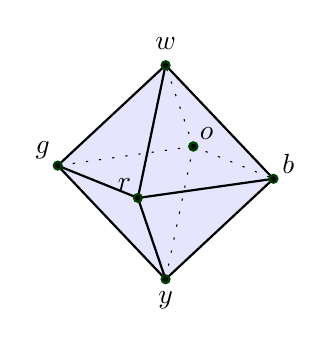
\begin{tikzpicture}%
  [x={(-0.860769cm, -0.121512cm)},
  y={(0.508996cm, -0.205391cm)},
  z={(-0.000053cm, 0.971107cm)},
  scale=1,
  back/.style={loosely dotted, thin},
  edge/.style={black, thick},
  facet/.style={fill=blue!95!black,fill opacity=0.1},
  vertex/.style={inner sep=1pt,circle,draw=green!25!black,fill=black,thick}]
\coordinate (-1, -1, 0) at (-1, -1, 0);
\coordinate (-1, 1, 0) at (-1, 1, 0);
\coordinate (0, 0, -1) at (0, 0, -1);
\coordinate (0, 0, 1) at (0, 0, 1);
\coordinate (1, -1, 0) at (1, -1, 0);
\coordinate (1, 1, 0) at (1, 1, 0);
%% Drawing edges in the back
%%
\draw[edge,back] (-1, -1, 0) -- (-1, 1, 0);
\draw[edge,back] (-1, -1, 0) -- (0, 0, -1.4);
\draw[edge,back] (-1, -1, 0) -- (0, 0, 1.4);
\draw[edge,back] (-1, -1, 0) -- (1, -1, 0);
%% Drawing vertices in the back
%%
\node[vertex] at (-1, -1, 0)     {};
%% Drawing the facets
%%
\fill[facet] (1, 1, 0) -- (0, 0, -1.4) -- (1, -1, 0) -- cycle {};
\fill[facet] (1, 1, 0) -- (0, 0, 1.4) -- (1, -1, 0) -- cycle {};
\fill[facet] (1, 1, 0) -- (-1, 1, 0) -- (0, 0, 1.4) -- cycle {};
\fill[facet] (1, 1, 0) -- (-1, 1, 0) -- (0, 0, -1.4) -- cycle {};
%% Drawing edges in the front
%%
\draw[edge] (-1, 1, 0) -- (0, 0, -1.4);
\draw[edge] (-1, 1, 0) -- (0, 0, 1.4);
\draw[edge] (-1, 1, 0) -- (1, 1, 0);
\draw[edge] (0, 0, -1.4) -- (1, -1, 0);
\draw[edge] (0, 0, -1.4) -- (1, 1, 0);
\draw[edge] (0, 0, 1.4) -- (1, -1, 0);
\draw[edge] (0, 0, 1.4) -- (1, 1, 0);
\draw[edge] (1, -1, 0) -- (1, 1, 0);
%% Drawing the vertices in the front
%%
\begin{scope}[nodes=vertex]
\node[label=above right:\( b \)] at (-1, 1, 0)     {};
\node[label=below:\( y \)] at (0, 0, -1.4)     {};
\node[label=above:\( w \)] at (0, 0, 1.4)     {};
\node[label=above left:\( g \)] at (1, -1, 0)     {};
\node[label=above left:\( r \)] at (1, 1, 0)     {};
\node[label=above right:\( o \)] at (-1, -1, 0)     {};
\end{scope}
\end{tikzpicture}
\caption{The HIT \( \oo \) which has 6 points, 12 1-paths, 8 2-paths.}
\end{figure}

We will choose a base point of \( \BAutoso \) that has four points, just like the equator of \( \oo \).

\begin{mydef}
Denote by \( C_4 \) the join \( \{b, g\}*\{r, o\} \). This is the equator of the discrete octahedral sphere. Then \( \oo \) itself can be seen as the join \( \{w, y\}* C_4 \).
\end{mydef}

\begin{figure}[h]
\centering
\begin{tikzpicture}[
node distance = 15mm and 15mm,
V/.style = {circle, fill, draw=black, inner sep=1pt, font=\footnotesize},
every edge quotes/.style = {auto, font=\footnotesize},
arrow/.style={->,semithick}
]
\begin{scope}[nodes=V]
  \node[label=above left:\( b \)] (1) {};
  \node[label=above right:\( r \)] (2) [right=of 1]  {};
  \node[label=below right:\( g \)] (3) [below=of 2]  {};
  \node[label=below left:\( o \)] (4) [below=of 1]  {};
\end{scope}
\draw[arrow]
        (1)  edge["\( br \)"] (2)
        (2)  edge["\( rg \)"] (3)
        (3)  edge["\( go \)"] (4)
        (4)  edge["\( ob \)"] (1);
\end{tikzpicture}
\caption{The HIT \( C_4 \) which is one of the types in \( \BAutoso \)}
\end{figure}

\begin{mylemma}
\( (C_4, b)\simeq S^1 \).
\end{mylemma}
\begin{proof}Similar to Lemma 6.5.1 from the HoTT book\cite{hottbook}. We will make some use of the particular map \( \{b, r, g, o\}\mapsto \mathsf{base}, br\mapsto \mathsf{loop}, \{rg, go, ob\}\mapsto \refl. \)\end{proof}

\begin{mylemma}
\( \oo\simeq S^2 \).
\end{mylemma}
\begin{proof}\( \oo \) is the join of \( C_4 \) and a two-point type. For more discussion of the join operation see the HoTT book section 8.5\cite{hottbook}.\end{proof}

To produce a term in \( \BAutoso \) we need \( C_4 \) and a choice of an equivalence class of equivalences with \( S^1 \):
\begin{mylemma}
We have \( (C_4, ||\{b, r, g, o\}\mapsto \mathsf{base}, br\mapsto \mathsf{loop}, \{rg, go, ob\}\mapsto \refl ||_0):\BAutoso \)
\end{mylemma}

There are other near-to-hand terms of \( \BAutoso \) we can denote like: \( [w, o, y, r] \), meaning the square isomorphic to \( C_4 \) but with the given four points, with pointing given by whichever point we listed first, and with equivalence with \( S^1 \) chosen so that the path between the first two points maps to \( \mathsf{loop} \). We will also introduce notation for maps \( f:[a, b, c, d]\to [w, x, y, z] \) by indicating where each item in the domain list is sent, like so: \( f\defeq[[x, y, z, w]] \).

\( C_4 \) has an unpointed automorphism connected to the identiy which will play the role of rotation by 90 degrees:

\begin{mydef}
Let \( R:C_4\to C_4 \) be the cyclic permutation given by \( R(b)=r, R(r)=g, R(g)=o, R(o)=b, R(br)=rg, R(rg)=go, R(go)=ob, R(ob)=br. \) Let \( R':R=\id \) be the obvious homotopy to the identity.
\end{mydef}

To construct a map \( \oo\to\BAutoso \) we need to send each vertex to an \( S^1 \)-torsor such as \( C_4 \). We will choose to send each vertex to ``the clockwise equator if this was the north pole.'' 

\begin{figure}[h]
\centering
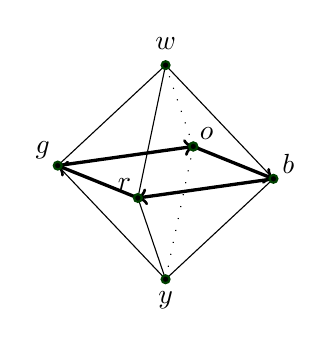
\begin{tikzpicture}%
  [x={(-0.860769cm, -0.121512cm)},
  y={(0.508996cm, -0.205391cm)},
  z={(-0.000053cm, 0.971107cm)},
  scale=1,
  eqback/.style={->, very thick},
  back/.style={loosely dotted, thin},
  eqedge/.style={->, very thick},
  edge/.style={black, thin},
  facet/.style={fill=blue!95!black,fill opacity=0.0},
  vertex/.style={inner sep=1pt,circle,draw=green!25!black,fill=black,thick}]
\coordinate (-1, -1, 0) at (-1, -1, 0);
\coordinate (-1, 1, 0) at (-1, 1, 0);
\coordinate (0, 0, -1) at (0, 0, -1);
\coordinate (0, 0, 1) at (0, 0, 1);
\coordinate (1, -1, 0) at (1, -1, 0);
\coordinate (1, 1, 0) at (1, 1, 0);
%% Drawing edges in the back
%%
\draw[edge,eqback] (-1, -1, 0) -- (-1, 1, 0);
\draw[edge,back] (-1, -1, 0) -- (0, 0, -1.4);
\draw[edge,back] (-1, -1, 0) -- (0, 0, 1.4);
\draw[edge,eqback] (1, -1, 0) -- (-1, -1, 0);
%% Drawing vertices in the back
%%
\node[vertex] at (-1, -1, 0)     {};
%% Drawing the facets
%%
\fill[facet] (1, 1, 0) -- (0, 0, -1.4) -- (1, -1, 0) -- cycle {};
\fill[facet] (1, 1, 0) -- (0, 0, 1.4) -- (1, -1, 0) -- cycle {};
\fill[facet] (1, 1, 0) -- (-1, 1, 0) -- (0, 0, 1.4) -- cycle {};
\fill[facet] (1, 1, 0) -- (-1, 1, 0) -- (0, 0, -1.4) -- cycle {};
%% Drawing edges in the front
%%
\draw[edge] (-1, 1, 0) -- (0, 0, -1.4);
\draw[edge] (-1, 1, 0) -- (0, 0, 1.4);
\draw[eqedge] (-1, 1, 0) -- (1, 1, 0);
\draw[edge] (0, 0, -1.4) -- (1, -1, 0);
\draw[edge] (0, 0, -1.4) -- (1, 1, 0);
\draw[edge] (0, 0, 1.4) -- (1, -1, 0);
\draw[edge] (0, 0, 1.4) -- (1, 1, 0);
\draw[eqedge] (1, 1, 0) -- (1, -1, 0);
%% Drawing the vertices in the front
%%
\begin{scope}[nodes=vertex]
\node[label=above right:\( b \)] at (-1, 1, 0)     {};
\node[label=below:\( y \)] at (0, 0, -1.4)     {};
\node[label=above:\( w \)] at (0, 0, 1.4)     {};
\node[label=above left:\( g \)] at (1, -1, 0)     {};
\node[label=above left:\( r \)] at (1, 1, 0)     {};
\node[label=above right:\( o \)] at (-1, -1, 0)     {};
\end{scope}
\end{tikzpicture}

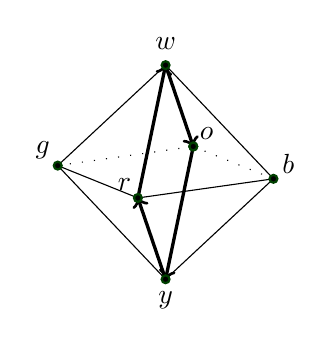
\begin{tikzpicture}%
  [x={(-0.860769cm, -0.121512cm)},
  y={(0.508996cm, -0.205391cm)},
  z={(-0.000053cm, 0.971107cm)},
  scale=1,
  eqback/.style={->, very thick},
  back/.style={loosely dotted, thin},
  eqedge/.style={->, very thick},
  edge/.style={black, thin},
  facet/.style={fill=blue!95!black,fill opacity=0.0},
  vertex/.style={inner sep=1pt,circle,draw=green!25!black,fill=black,thick}]
\coordinate (-1, -1, 0) at (-1, -1, 0);
\coordinate (-1, 1, 0) at (-1, 1, 0);
\coordinate (0, 0, -1) at (0, 0, -1);
\coordinate (0, 0, 1) at (0, 0, 1);
\coordinate (1, -1, 0) at (1, -1, 0);
\coordinate (1, 1, 0) at (1, 1, 0);
%% Drawing edges in the back
%%
\draw[edge,back] (-1, -1, 0) -- (-1, 1, 0);
\draw[edge,eqback] (-1, -1, 0) -- (0, 0, -1.4);
\draw[edge,eqback] (0, 0, 1.4) -- (-1, -1, 0);
\draw[edge,back] (1, -1, 0) -- (-1, -1, 0);
%% Drawing vertices in the back
%%
\node[vertex] at (-1, -1, 0)     {};
%% Drawing the facets
%%
\fill[facet] (1, 1, 0) -- (0, 0, -1.4) -- (1, -1, 0) -- cycle {};
\fill[facet] (1, 1, 0) -- (0, 0, 1.4) -- (1, -1, 0) -- cycle {};
\fill[facet] (1, 1, 0) -- (-1, 1, 0) -- (0, 0, 1.4) -- cycle {};
\fill[facet] (1, 1, 0) -- (-1, 1, 0) -- (0, 0, -1.4) -- cycle {};
%% Drawing edges in the front
%%
\draw[edge] (-1, 1, 0) -- (0, 0, -1.4);
\draw[edge] (-1, 1, 0) -- (0, 0, 1.4);
\draw[edge] (-1, 1, 0) -- (1, 1, 0);
\draw[edge] (0, 0, -1.4) -- (1, -1, 0);
\draw[eqedge] (0, 0, -1.4) -- (1, 1, 0);
\draw[edge] (0, 0, 1.4) -- (1, -1, 0);
\draw[eqedge] (1, 1, 0) -- (0, 0, 1.4) ;
\draw[edge] (1, 1, 0) -- (1, -1, 0);
%% Drawing the vertices in the front
%%
\begin{scope}[nodes=vertex]
\node[label=above right:\( b \)] at (-1, 1, 0)     {};
\node[label=below:\( y \)] at (0, 0, -1.4)     {};
\node[label=above:\( w \)] at (0, 0, 1.4)     {};
\node[label=above left:\( g \)] at (1, -1, 0)     {};
\node[label=above left:\( r \)] at (1, 1, 0)     {};
\node[label=above right:\( o \)] at (-1, -1, 0)     {};
\end{scope}
\end{tikzpicture}

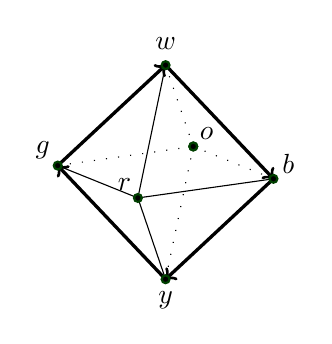
\begin{tikzpicture}%
  [x={(-0.860769cm, -0.121512cm)},
  y={(0.508996cm, -0.205391cm)},
  z={(-0.000053cm, 0.971107cm)},
  scale=1,
  eqback/.style={->, very thick},
  back/.style={loosely dotted, thin},
  eqedge/.style={->, very thick},
  edge/.style={black, thin},
  facet/.style={fill=blue!95!black,fill opacity=0.0},
  vertex/.style={inner sep=1pt,circle,draw=green!25!black,fill=black,thick}]
\coordinate (-1, -1, 0) at (-1, -1, 0);
\coordinate (-1, 1, 0) at (-1, 1, 0);
\coordinate (0, 0, -1) at (0, 0, -1);
\coordinate (0, 0, 1) at (0, 0, 1);
\coordinate (1, -1, 0) at (1, -1, 0);
\coordinate (1, 1, 0) at (1, 1, 0);
%% Drawing edges in the back
%%
\draw[edge,back] (-1, -1, 0) -- (-1, 1, 0);
\draw[edge,back] (-1, -1, 0) -- (0, 0, -1.4);
\draw[edge,back] (-1, -1, 0) -- (0, 0, 1.4);
\draw[edge,back] (1, -1, 0) -- (-1, -1, 0);
%% Drawing vertices in the back
%%
\node[vertex] at (-1, -1, 0)     {};
%% Drawing the facets
%%
\fill[facet] (1, 1, 0) -- (0, 0, -1.4) -- (1, -1, 0) -- cycle {};
\fill[facet] (1, 1, 0) -- (0, 0, 1.4) -- (1, -1, 0) -- cycle {};
\fill[facet] (1, 1, 0) -- (-1, 1, 0) -- (0, 0, 1.4) -- cycle {};
\fill[facet] (1, 1, 0) -- (-1, 1, 0) -- (0, 0, -1.4) -- cycle {};
%% Drawing edges in the front
%%
\draw[eqedge] (-1, 1, 0) -- (0, 0, -1.4);
\draw[eqedge] (0, 0, 1.4) -- (-1, 1, 0);
\draw[edge] (-1, 1, 0) -- (1, 1, 0);
\draw[eqedge] (0, 0, -1.4) -- (1, -1, 0);
\draw[edge] (0, 0, -1.4) -- (1, 1, 0);
\draw[eqedge] (1, -1, 0) -- (0, 0, 1.4);
\draw[edge] (0, 0, 1.4) -- (1, 1, 0);
\draw[edge] (1, 1, 0) -- (1, -1, 0);
%% Drawing the vertices in the front
%%
\begin{scope}[nodes=vertex]
\node[label=above right:\( b \)] at (-1, 1, 0)     {};
\node[label=below:\( y \)] at (0, 0, -1.4)     {};
\node[label=above:\( w \)] at (0, 0, 1.4)     {};
\node[label=above left:\( g \)] at (1, -1, 0)     {};
\node[label=above left:\( r \)] at (1, 1, 0)     {};
\node[label=above right:\( o \)] at (-1, -1, 0)     {};
\end{scope}
\end{tikzpicture}
\caption{The equators for \( w, b, r \).}
\end{figure}

\begin{mydef}
Define \( T_0:\oo\to\BAutoso \) on just the 0-skeleton by
\begin{itemize}
\item \( T_0(b)=[w, o, y, r] \).
\item \( T_0(o)=[w, g, y, b] \).
\item \( T_0(g)=[w, r, y, o] \).
\item \( T_0(r)=[w, b, y, g] \).
\item \( T_0(w)=[b, r, g, o] \).
\item \( T_0(y)=[b, o, g, r] \).
\end{itemize}
\end{mydef}

Extending this to the 1-skeleton requires various choices. We will choose the one that reflects the tangent bundle, using the transport we can intuitively see through the embedding of \( \oo \) in 3-dimensional space as in our pictures. If you focus for a moment just on a path \( w\to b\to r \) and imagine rigidly tipping a moving equator along with a moving point, you can imagine a moving-equator point that starts at \( r \) and stays fixed when the north pole slides from \( w \) to \( b \). When the north pole continues sliding from \( b \) to \( r \) the moving-equator point moves to \( g \). Then it remains fixed when the north pole slides from \( r \) up to \( w \). So all in all we ``moved \( r \) to \( g \).'' When we track all the points on the original \( w \)-equator we see that we performed the rotation we earlier named \( R \).

In general we have:
\begin{mydef}
Define \( T_1:\oo\to\BAutoso \) on just the 1-skeleton by extending \( T_0 \) as follows:
Transport away from \( w \):
\begin{itemize}
\item \( T_1(wb):[b, r, g, o]\mapsto [y, r, w, o] \) (\( r, o \) fixed)
\item \( T_1(wr):[b, r, g, o]\mapsto [b, y, g, w] \) (\( b, g \) fixed)
\item \( T_1(wg):[b, r, g, o]\mapsto [w, r, y, o] \)
\item \( T_1(wo):[b, r, g, o]\mapsto [b, w, g, y] \)
\end{itemize}
Transport away from \( y \):
\begin{itemize}
\item \( T_1(yb):[b, o, g, r]\mapsto [w, o, y, r] \)
\item \( T_1(yr):[b, o, g, r]\mapsto [b, y, g, w] \)
\item \( T_1(yg):[b, o, g, r]\mapsto [y, o, w, r] \)
\item \( T_1(yo):[b, o, g, r]\mapsto [b, w, g, y] \)
\end{itemize}
Transport along the equator:
\begin{itemize}
\item \( T_1(br):[w, o, y, r]\mapsto [w, b, y, g] \) 
\item \( T_1(rg):[w, b, y, g]\mapsto [w, r, y, o] \)
\item \( T_1(go):[w, r, y, o]\mapsto [w, g, y, b] \)
\item \( T_1(ob):[w, g, y, b]\mapsto [w, o, y, r] \)
\end{itemize}
\end{mydef}

At this point we have defined a map on the 1-skeleton of \( \oo \).

\begin{myclaim}
\( T_1 \) defines a principal circle bundle with connection over the 1-skeleton of \( \oo \).
\end{myclaim}

We now want to extend this map to all of \( \oo \) by providing values for the eight faces. Here we will be guided by the classical relationship between a connection and its curvature. The curvature is computed from the connection, it doesn't contain any new data. Classically the integral of curvature over a 2-cell is the holonomy given by transport around the boundary. 

\begin{mydef}
Define \( T_2:\oo\to\BAutoso \) by extending \( T_1 \) as follows. We will send every clockwise triangle to \( R' \), the homotopy from \( \refl \) to \( R \):
\begin{itemize}
\item \( T_2(wbr)=R' \) 
\item \( T_2(wrg)=R' \)
\item \( T_2(wgo)=R' \)
\item \( T_2(ybo)=R' \)
\item \( T_2(yrb)=R' \) 
\item \( T_2(ygr)=R' \)
\item \( T_2(yog)=R' \)
\item \( T_2(ybo)=R' \)
\end{itemize}
\end{mydef}


\subsection{Combinatorial manifolds}

(This section is not quite off the ground.)

The combinatorial structure we have in mind is a nerve of a good open cover. What do we know about which smooth manifolds have such covers? While we're at it, let's survey all the combinatorial-flavored spaces and survey what smooth manifolds are homotopy equivalent to which structures.

What topological manifolds are equivalent to a CW complex? The answer is the composition of a few results summarized by Allen Hatcher\footnote{\url{https://mathoverflow.net/questions/201944/topological-n-manifolds-have-the-homotopy-type-of-n-dimensional-cw-complexes}} (citing \cite{kirby_siebenmann} and \cite{freedman_quinn}):

\begin{quote}
Every topological manifold has a handlebody structure except in dimension 4, where a 4-manifold has a handlebody structure if and only if it is smoothable. This is a theorem on page 136 of Freedman and Quinn's book ``Topology of 4-Manifolds'', with a reference given to the Kirby-Siebenmann book for the higher-dimensional case. It is then an elementary fact that an \( n \)-manifold with a handlebody structure is homotopy equivalent to a CW complex with one \( k \)-cell for each \( k \)-handle, so in particular there are no cells of dimension greater than \( n \). At least in the compact case a manifold with a handlebody structure is in fact homeomorphic to a CW complex with \( k \)-cells corresponding to \( k \)-handles; see page 107 of Kirby-Siebenmann. This probably holds in the noncompact case as well, though I don't know a reference.
\end{quote}




\section{Central H-spaces}

\begin{itemize}
\item introduce torsors
\item show subtlety how \( BG \) doesn't classify stuff since it has extra properties
\item draw 
% https://q.uiver.app/#q=WzAsNyxbMSwwLCJQIl0sWzIsMCwiRUciXSxbMywwLCJcXG1hdGhjYWx7VX0nIl0sWzEsMSwiTSJdLFsyLDEsIkJHIl0sWzMsMSwiXFxtYXRoY2Fse1V9Il0sWzAsMCwiXFxzdW1fe2E6TX1VKGYoeCkpIl0sWzQsNSwiVShcXHRleHR7Zm9yZ2V0fSkiXSxbMSwyXSxbMCwxXSxbMyw0LCJmIl0sWzAsM10sWzEsNF0sWzIsNV0sWzAsNCwiIiwwLHsic3R5bGUiOnsibmFtZSI6ImNvcm5lciJ9fV0sWzEsNSwiIiwwLHsic3R5bGUiOnsibmFtZSI6ImNvcm5lciJ9fV0sWzYsMCwiOj0iXV0=
\begin{tikzcd}
  {\sum_{a:M}U(f(x))} & P & EG & {\mathcal{U}'} \\
  & M & BG & {\mathcal{U}}
  \arrow["{:=}", from=1-1, to=1-2]
  \arrow[from=1-2, to=1-3]
  \arrow[from=1-2, to=2-2]
  \arrow["\lrcorner"{anchor=center, pos=0.125}, draw=none, from=1-2, to=2-3]
  \arrow[from=1-3, to=1-4]
  \arrow[from=1-3, to=2-3]
  \arrow["\lrcorner"{anchor=center, pos=0.125}, draw=none, from=1-3, to=2-4]
  \arrow[from=1-4, to=2-4]
  \arrow["f", from=2-2, to=2-3]
  \arrow["{U(\text{forget})}", from=2-3, to=2-4]
\end{tikzcd}
\item H-spaces paper result equating this to a universal cover of a component of the universe. (It should feel significant that \( BS^1\simeq \BAutoso \).)
\end{itemize}

To create a tangent bundle of a surface we need to map loops on the surface to isomorphisms of the plane. For us this means we need to map loops on the surface to circles. That in turn means we are looking for a codomain that is a \emph{delooping} of the circle.

Let \( G \) be a group consisting of a set (0-type) \( S \), an identity \( e:S \), a multiplication \( \mu:S\times S \to S \), an inverse function \( i:S\to S \) satisfying the group laws (associativity of \( \mu \), unit laws). 

Let a \( G \)-type be a type \( X:\U \) equipped with an action \( m:G\to X\simeq X \). To form a classifying type \( \GType \) of \( G \)-types we can let \( G \) act on the universe:

% https://q.uiver.app/#q=WzAsMyxbMCwwLCJHXFx0aW1lc1xcbWF0aGNhbHtVfV8qIl0sWzAsMSwiXFxtYXRoY2Fse1V9XyoiXSxbMCwyLCJcXG1hdGhjYWx7VX0iXSxbMCwxLCJtIl0sWzEsMiwiXFxtYXRocm17cHJ9XzEiXV0=
\begin{center}
\begin{tikzcd}
  {G\times\mathcal{U}_*} \\
  {\mathcal{U}_*} \\
  {\mathcal{U}}
  \arrow["m", from=1-1, to=2-1]
  \arrow["{\mathrm{pr}_1}", from=2-1, to=3-1]
\end{tikzcd}
\end{center}

where \( m \) preserves fibers of the universal fibration. We can form type families of \( G \)-types by pulling back this diagram:

% https://q.uiver.app/#q=WzAsNixbMSwwLCJHXFx0aW1lc1xcbWF0aGNhbHtVfV8qIl0sWzEsMSwiXFxtYXRoY2Fse1V9XyoiXSxbMSwyLCJcXG1hdGhjYWx7VX0iXSxbMCwwLCJHXFx0aW1lcyBQIl0sWzAsMSwiUCJdLFswLDIsIlgiXSxbMCwxLCJtIl0sWzEsMiwiXFxtYXRocm17cHJ9XzEiXSxbNCw1LCJcXG1hdGhybXtwcn1fMSIsMl0sWzMsNCwibSIsMl0sWzMsMF0sWzQsMV0sWzUsMl0sWzQsMiwiIiwyLHsic3R5bGUiOnsibmFtZSI6ImNvcm5lciJ9fV0sWzMsMSwiIiwyLHsic3R5bGUiOnsibmFtZSI6ImNvcm5lciJ9fV1d
\begin{center}
\begin{tikzcd}
  {G\times P} & {G\times\mathcal{U}_*} \\
  P & {\mathcal{U}_*} \\
  X & {\mathcal{U}}
  \arrow[from=1-1, to=1-2]
  \arrow["m"', from=1-1, to=2-1]
  \arrow["\lrcorner"{anchor=center, pos=0.125}, draw=none, from=1-1, to=2-2]
  \arrow["m", from=1-2, to=2-2]
  \arrow[from=2-1, to=2-2]
  \arrow["{\mathrm{pr}_1}"', from=2-1, to=3-1]
  \arrow["\lrcorner"{anchor=center, pos=0.125}, draw=none, from=2-1, to=3-2]
  \arrow["{\mathrm{pr}_1}", from=2-2, to=3-2]
  \arrow[from=3-1, to=3-2]
\end{tikzcd}
\end{center}

If we add to this the requirement that the action be free and transitive, we obtain the type \( \GTor \) of \( G \)-torsors.

Central H-spaces are the classifying spaces for principal bundles on abelian groups. We won't be able to access the full theory for nonabelian groups just yet, but we hope that the theory of maximal tori and weights might bring even those within reach of the central H-space paradigm.

We will rely on the lovely paper by Buchholtz, Christensen, Flaten and Rijke \cite{buchholtz2023central}. 

\begin{mydef}
An H-space structure on a pointed type \( (B,b) \) consists of
\begin{enumerate}
\item A binary operation \( \mu:B\to B\to B \)
\item A left unit law \( \mu_l:\mu(\pt,-)=\id_B \)
\item A right unit law \( \mu_r:\mu(-,\pt)=\id_B \)
\item A coherence \( \mu_{lr}:\mu_l(\pt)=_{\mu(\pt,\pt)=\pt}\mu_r(\pt) \)
\item A proof of left- and right- invertibility: \( \mu(a,-):A\simeq A \), \( \mu(-, b):A\simeq A \)
\end{enumerate}
\end{mydef}

\begin{myprop}
(\cite{buchholtz2023central} Prop 3.6) Let \( A \) be a pointed type. Then the following are equivalent:
\begin{enumerate}
\item \( A \) is central.
\item \( A \) is a connected H-space and \( A\dotto A \) is a set.
\item \( A \) is a connected H-space and \( A\simeq A \) is a set.
\end{enumerate}
\end{myprop}

This result will inform our study of the Leibniz rule: the analogue of the algebra of functions to \( \rr \) is:
\begin{myprop}
For any type \( M \) and H-space \( B \) the type of maps \( M\to B \) with base point the constant map is an H-space under pointwise multiplication.
\end{myprop}

We will also be looking in detail at maps into the classifying space of \( S^1 \) bundles. The Buchholtz et al paper\cite{buchholtz2023central} describes this type in several helpful ways, summarized by:

\begin{mythm}
For any central H-space \( A \) (such as \( S^1 \)) the type of torsors of \( A \) is a delooping of \( A \), and is equivalent to \( \BAut_1(A)\defeq \sit{X:\U}||X=A||_0. \) This delooping is also a central H-space and so can be infinitely delooped.
\end{mythm}

This means that we can form a sequence of deloopings \( \zz, S^1, \BAutoso, \ldots \).





\section{Connections and curvature}

\subsection{The function \texorpdfstring{\( T \)}{T}}

We will build up a map \( T \) out of \( \oo \) which is meant to be like the circle bundle of a tangent bundle. And so we will begin with the intrinsic data of the link at each point: taking the link of a vertex gives us a map from vertices to polygons.

\begin{mydef}
\( T_0\defeq\link:\oo_0\to\EMzo \) is given by:
\begin{align*}
\link(w) &= brgo & \link(r) &= wbyg \\
\link(y) &= bogr & \link(g) &= wryo \\
\link(b) &= woyr & \link(o) &= wgyb
\end{align*}
We chose these orderings for the vertices in the link, by visualizing standing at the given vertex as if it were the north pole, then looking south and enumerating the link in clockwise order, starting from \( w \) if possible, else \( b \).
\end{mydef}

\begin{figure}[htbp]
\centering
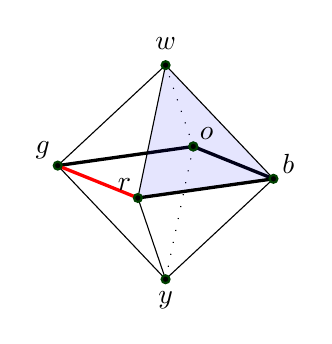
\begin{tikzpicture}%
  [x={(-0.860769cm, -0.121512cm)},
  y={(0.508996cm, -0.205391cm)},
  z={(-0.000053cm, 0.971107cm)},
  scale=1,
  eqback/.style={very thick},
  back/.style={loosely dotted, thin},
  eqedge/.style={very thick},
  edge/.style={black, thin},
  r/.style={red},
  facet/.style={fill=blue!95!black,fill opacity=0.1},
  vertex/.style={inner sep=1pt,circle,draw=green!25!black,fill=black,thick}]
\coordinate (-1, -1, 0) at (-1, -1, 0);
\coordinate (-1, 1, 0) at (-1, 1, 0);
\coordinate (0, 0, -1) at (0, 0, -1);
\coordinate (0, 0, 1) at (0, 0, 1);
\coordinate (1, -1, 0) at (1, -1, 0);
\coordinate (1, 1, 0) at (1, 1, 0);
%% Drawing edges in the back
%%
\draw[edge,eqback] (-1, -1, 0) -- (-1, 1, 0);
\draw[edge,back] (-1, -1, 0) -- (0, 0, -1.4);
\draw[edge,back] (-1, -1, 0) -- (0, 0, 1.4);
\draw[edge,eqback] (1, -1, 0) -- (-1, -1, 0);
%% Drawing vertices in the back
%%
\node[vertex] at (-1, -1, 0)     {};
%% Drawing the facets
%%
%\fill[facet] (1, 1, 0) -- (0, 0, -1.4) -- (1, -1, 0) -- cycle {};
%\fill[facet] (1, 1, 0) -- (0, 0, 1.4) -- (1, -1, 0) -- cycle {};
\fill[facet] (1, 1, 0) -- (-1, 1, 0) -- (0, 0, 1.4) -- cycle {};
%\fill[facet] (1, 1, 0) -- (-1, 1, 0) -- (0, 0, -1.4) -- cycle {};
%% Drawing edges in the front
%%
\draw[edge] (-1, 1, 0) -- (0, 0, -1.4);
\draw[edge] (-1, 1, 0) -- (0, 0, 1.4);
\draw[eqedge] (-1, 1, 0) -- (1, 1, 0);
\draw[edge] (0, 0, -1.4) -- (1, -1, 0);
\draw[edge] (0, 0, -1.4) -- (1, 1, 0);
\draw[edge] (0, 0, 1.4) -- (1, -1, 0);
\draw[edge] (0, 0, 1.4) -- (1, 1, 0);
\draw[r,eqedge] (1, 1, 0) -- (1, -1, 0);
%% Drawing the vertices in the front
%%
\begin{scope}[nodes=vertex]
\node[label=above right:\( b \)] at (-1, 1, 0)     {};
\node[label=below:\( y \)] at (0, 0, -1.4)     {};
\node[label=above:\( w \)] at (0, 0, 1.4)     {};
\node[label=above left:\( g \)] at (1, -1, 0)     {};
\node[label=above left:\( r \)] at (1, 1, 0)     {};
\node[label=above right:\( o \)] at (-1, -1, 0)     {};
\end{scope}
\end{tikzpicture}
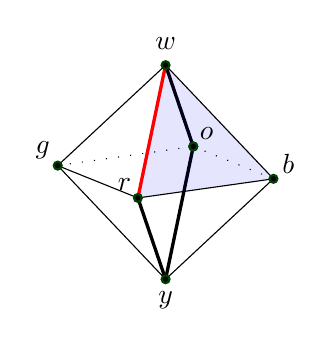
\begin{tikzpicture}%
  [x={(-0.860769cm, -0.121512cm)},
  y={(0.508996cm, -0.205391cm)},
  z={(-0.000053cm, 0.971107cm)},
  scale=1,
  eqback/.style={very thick},
  back/.style={loosely dotted, thin},
  eqedge/.style={very thick},
  r/.style={red},
  edge/.style={black, thin},
  facet/.style={fill=blue!95!black,fill opacity=0.1},
  vertex/.style={inner sep=1pt,circle,draw=green!25!black,fill=black,thick}]
\coordinate (-1, -1, 0) at (-1, -1, 0);
\coordinate (-1, 1, 0) at (-1, 1, 0);
\coordinate (0, 0, -1) at (0, 0, -1);
\coordinate (0, 0, 1) at (0, 0, 1);
\coordinate (1, -1, 0) at (1, -1, 0);
\coordinate (1, 1, 0) at (1, 1, 0);
%% Drawing edges in the back
%%
\draw[edge,back] (-1, -1, 0) -- (-1, 1, 0);
\draw[edge,eqback] (-1, -1, 0) -- (0, 0, -1.4);
\draw[edge,eqback] (0, 0, 1.4) -- (-1, -1, 0);
\draw[edge,back] (1, -1, 0) -- (-1, -1, 0);
%% Drawing vertices in the back
%%
\node[vertex] at (-1, -1, 0)     {};
%% Drawing the facets
%%
% \fill[facet] (1, 1, 0) -- (0, 0, -1.4) -- (1, -1, 0) -- cycle {};
% \fill[facet] (1, 1, 0) -- (0, 0, 1.4) -- (1, -1, 0) -- cycle {};
\fill[facet] (1, 1, 0) -- (-1, 1, 0) -- (0, 0, 1.4) -- cycle {};
% \fill[facet] (1, 1, 0) -- (-1, 1, 0) -- (0, 0, -1.4) -- cycle {};
%% Drawing edges in the front
%%
\draw[edge] (-1, 1, 0) -- (0, 0, -1.4);
\draw[edge] (-1, 1, 0) -- (0, 0, 1.4);
\draw[edge] (-1, 1, 0) -- (1, 1, 0);
\draw[edge] (0, 0, -1.4) -- (1, -1, 0);
\draw[eqedge] (0, 0, -1.4) -- (1, 1, 0);
\draw[edge] (0, 0, 1.4) -- (1, -1, 0);
\draw[r,eqedge] (1, 1, 0) -- (0, 0, 1.4) ;
\draw[edge] (1, 1, 0) -- (1, -1, 0);
%% Drawing the vertices in the front
%%
\begin{scope}[nodes=vertex]
\node[label=above right:\( b \)] at (-1, 1, 0)     {};
\node[label=below:\( y \)] at (0, 0, -1.4)     {};
\node[label=above:\( w \)] at (0, 0, 1.4)     {};
\node[label=above left:\( g \)] at (1, -1, 0)     {};
\node[label=above left:\( r \)] at (1, 1, 0)     {};
\node[label=above right:\( o \)] at (-1, -1, 0)     {};
\end{scope}
\end{tikzpicture}
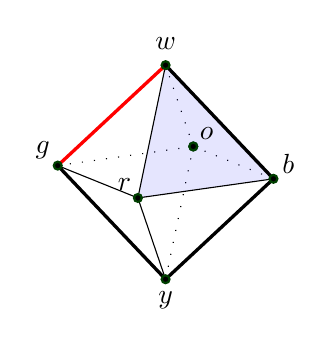
\begin{tikzpicture}%
  [x={(-0.860769cm, -0.121512cm)},
  y={(0.508996cm, -0.205391cm)},
  z={(-0.000053cm, 0.971107cm)},
  scale=1,
  eqback/.style={very thick},
  back/.style={loosely dotted, thin},
  eqedge/.style={very thick},
  r/.style={red},
  edge/.style={black, thin},
  facet/.style={fill=blue!95!black,fill opacity=0.1},
  vertex/.style={inner sep=1pt,circle,draw=green!25!black,fill=black,thick}]
\coordinate (-1, -1, 0) at (-1, -1, 0);
\coordinate (-1, 1, 0) at (-1, 1, 0);
\coordinate (0, 0, -1) at (0, 0, -1);
\coordinate (0, 0, 1) at (0, 0, 1);
\coordinate (1, -1, 0) at (1, -1, 0);
\coordinate (1, 1, 0) at (1, 1, 0);
%% Drawing edges in the back
%%
\draw[edge,back] (-1, -1, 0) -- (-1, 1, 0);
\draw[edge,back] (-1, -1, 0) -- (0, 0, -1.4);
\draw[edge,back] (-1, -1, 0) -- (0, 0, 1.4);
\draw[edge,back] (1, -1, 0) -- (-1, -1, 0);
%% Drawing vertices in the back
%%
\node[vertex] at (-1, -1, 0)     {};
%% Drawing the facets
%%
% \fill[facet] (1, 1, 0) -- (0, 0, -1.4) -- (1, -1, 0) -- cycle {};
% \fill[facet] (1, 1, 0) -- (0, 0, 1.4) -- (1, -1, 0) -- cycle {};
\fill[facet] (1, 1, 0) -- (-1, 1, 0) -- (0, 0, 1.4) -- cycle {};
% \fill[facet] (1, 1, 0) -- (-1, 1, 0) -- (0, 0, -1.4) -- cycle {};
%% Drawing edges in the front
%%
\draw[eqedge] (-1, 1, 0) -- (0, 0, -1.4);
\draw[eqedge] (0, 0, 1.4) -- (-1, 1, 0);
\draw[edge] (-1, 1, 0) -- (1, 1, 0);
\draw[eqedge] (0, 0, -1.4) -- (1, -1, 0);
\draw[edge] (0, 0, -1.4) -- (1, 1, 0);
\draw[r,eqedge] (1, -1, 0) -- (0, 0, 1.4);
\draw[edge] (0, 0, 1.4) -- (1, 1, 0);
\draw[edge] (1, 1, 0) -- (1, -1, 0);
%% Drawing the vertices in the front
%%
\begin{scope}[nodes=vertex]
\node[label=above right:\( b \)] at (-1, 1, 0)     {};
\node[label=below:\( y \)] at (0, 0, -1.4)     {};
\node[label=above:\( w \)] at (0, 0, 1.4)     {};
\node[label=above left:\( g \)] at (1, -1, 0)     {};
\node[label=above left:\( r \)] at (1, 1, 0)     {};
\node[label=above right:\( o \)] at (-1, -1, 0)     {};
\end{scope}
\end{tikzpicture}
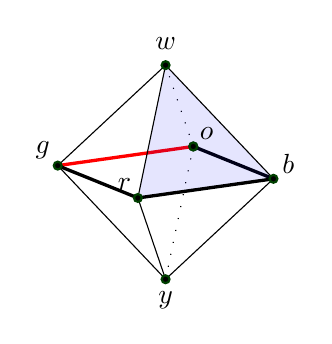
\begin{tikzpicture}%
  [x={(-0.860769cm, -0.121512cm)},
  y={(0.508996cm, -0.205391cm)},
  z={(-0.000053cm, 0.971107cm)},
  scale=1,
  eqback/.style={very thick},
  back/.style={loosely dotted, thin},
  eqedge/.style={very thick},
  edge/.style={black, thin},
  r/.style={red},
  facet/.style={fill=blue!95!black,fill opacity=0.1},
  vertex/.style={inner sep=1pt,circle,draw=green!25!black,fill=black,thick}]
\coordinate (-1, -1, 0) at (-1, -1, 0);
\coordinate (-1, 1, 0) at (-1, 1, 0);
\coordinate (0, 0, -1) at (0, 0, -1);
\coordinate (0, 0, 1) at (0, 0, 1);
\coordinate (1, -1, 0) at (1, -1, 0);
\coordinate (1, 1, 0) at (1, 1, 0);
%% Drawing edges in the back
%%
\draw[edge,eqback] (-1, -1, 0) -- (-1, 1, 0);
\draw[edge,back] (-1, -1, 0) -- (0, 0, -1.4);
\draw[edge,back] (-1, -1, 0) -- (0, 0, 1.4);
\draw[edge,eqback,r] (1, -1, 0) -- (-1, -1, 0);
%% Drawing vertices in the back
%%
\node[vertex] at (-1, -1, 0)     {};
%% Drawing the facets
%%
% \fill[facet] (1, 1, 0) -- (0, 0, -1.4) -- (1, -1, 0) -- cycle {};
% \fill[facet] (1, 1, 0) -- (0, 0, 1.4) -- (1, -1, 0) -- cycle {};
\fill[facet] (1, 1, 0) -- (-1, 1, 0) -- (0, 0, 1.4) -- cycle {};
% \fill[facet] (1, 1, 0) -- (-1, 1, 0) -- (0, 0, -1.4) -- cycle {};
%% Drawing edges in the front
%%
\draw[edge] (-1, 1, 0) -- (0, 0, -1.4);
\draw[edge] (-1, 1, 0) -- (0, 0, 1.4);
\draw[eqedge] (-1, 1, 0) -- (1, 1, 0);
\draw[edge] (0, 0, -1.4) -- (1, -1, 0);
\draw[edge] (0, 0, -1.4) -- (1, 1, 0);
\draw[edge] (0, 0, 1.4) -- (1, -1, 0);
\draw[edge] (0, 0, 1.4) -- (1, 1, 0);
\draw[eqedge] (1, 1, 0) -- (1, -1, 0);
%% Drawing the vertices in the front
%%
\begin{scope}[nodes=vertex]
\node[label=above right:\( b \)] at (-1, 1, 0)     {};
\node[label=below:\( y \)] at (0, 0, -1.4)     {};
\node[label=above:\( w \)] at (0, 0, 1.4)     {};
\node[label=above left:\( g \)] at (1, -1, 0)     {};
\node[label=above left:\( r \)] at (1, 1, 0)     {};
\node[label=above right:\( o \)] at (-1, -1, 0)     {};
\end{scope}
\end{tikzpicture}

\caption{\( \link \) for the vertices \( w, b\) and \( r \).}
\label{fig:triangle_of_equators}
\end{figure}

To extend \( T_0 \) to a function \( T_1 \) on the 1-skeleton we have complete freedom. Defining a map by induction makes clear that the action on paths is its own structure. Two functions on the octahedron could agree on points but differ on edges. We are going to identify this 1-dimensional freedom with a connection:

\begin{mydef}
\label{def:connection}
A \defemph{connection} on a higher combinatorial manifold is an extension of a circle bundle from the 0-skeleton to the 1-skeleton.
\end{mydef}

Continuing the example, we will do something ``tangent bundley'', imagining how \( T_1 \) changes as we slide from point to point in the embedding shown in the figures. Sliding from \( w \) to \( b \) and tipping the link as we go, we see \( r\mapsto r \) and \( o\mapsto o \) because those lie on the axis of rotation. Then \( g\mapsto w \) and \( b\mapsto y \). 

\begin{mydef}
Define \( T_1:\oo_1\to\EMzo \) on just the 1-skeleton by extending \( T_0 \) as follows:
Transport away from \( w \):
\begin{itemize}
\item \( T_1(wb):[b, r, g, o]\mapsto [y, r, w, o] \) (\( r, o \) fixed)
\item \( T_1(wr):[b, r, g, o]\mapsto [b, y, g, w] \) (\( b, g \) fixed)
\item \( T_1(wg):[b, r, g, o]\mapsto [w, r, y, o] \)
\item \( T_1(wo):[b, r, g, o]\mapsto [b, w, g, y] \)
\end{itemize}
Transport away from \( y \):
\begin{itemize}
\item \( T_1(yb):[b, o, g, r]\mapsto [w, o, y, r] \)
\item \( T_1(yr):[b, o, g, r]\mapsto [b, y, g, w] \)
\item \( T_1(yg):[b, o, g, r]\mapsto [y, o, w, r] \)
\item \( T_1(yo):[b, o, g, r]\mapsto [b, w, g, y] \)
\end{itemize}
Transport along the equator:
\begin{itemize}
\item \( T_1(br):[w, o, y, r]\mapsto [w, b, y, g] \) 
\item \( T_1(rg):[w, b, y, g]\mapsto [w, r, y, o] \)
\item \( T_1(go):[w, r, y, o]\mapsto [w, g, y, b] \)
\item \( T_1(ob):[w, g, y, b]\mapsto [w, o, y, r] \)
\end{itemize}
\end{mydef}

It's very important to be able to visualize what \( T_1 \) does to triangular paths such as \( wb\cdot br\cdot rw \) (which circulates around the boundary of face \( wbr \)). You can see it if you imagine Figure~\ref{fig:triangle_of_equators} as the frames of a short movie. Or you can place your palm over the top of a cube and note where your fingers are pointing, then slide your hand to an equatorial face, then along the equator, then back to the top. The answer is: you come back rotated clockwise by a quarter-turn. 

\begin{mydef}
The map \( R:C_4\to C_4 \) rotates by one quarter turn, one ``click":
\begin{multicols}{2}
\begin{itemize}
\item \( R(c_1) = c_2 \)
\item \( R(c_2) = c_3 \)
\item \( R(c_3) = c_4 \)
\item \( R(c_4) = c_1 \)
\item \( R(c_1c_2) = c_2c_3 \)
\item \( R(c_2c_3) = c_3c_4 \)
\item \( R(c_3c_4) = c_4c_1 \)
\item \( R(c_4c_1) = c_1c_2 \)
\end{itemize}
\end{multicols}
\end{mydef}

Note by univalence the equivalence \( R \) gives a loop in the universe, a term of \( C_4=_{\EMzo}C_4 \).

Now let's extend \( T_1 \) to all of \( \oo \) by providing values for the eight faces. The face \( wbr \) is a path from \( \refl_w \) to the concatenation \( wb\cdot br\cdot rw \), and so the image of \( wbr \) under the extended version of \( T_1 \) must be a homotopy from \( \refl_{T_1(w)} \) to \( T_1(wb\cdot br\cdot rw) \). Here \emph{there is no additional freedom}.

\begin{mydef}
Define \( T_2:\oo\to\EMzo \) by extending \( T_1 \) to the faces as follows:
\begin{multicols}{2}
\begin{itemize}
\item \( T_2(wbr)=H_R \) 
\item \( T_2(wrg)=H_R \)
\item \( T_2(wgo)=H_R \)
\item \( T_2(ybo)=H_R \)
\item \( T_2(yrb)=H_R \) 
\item \( T_2(ygr)=H_R \)
\item \( T_2(yog)=H_R \)
\item \( T_2(ybo)=H_R \)
\end{itemize}
\end{multicols}
where \( H_R:R=\refl_{C_4} \) is the obvious homotopy given by composition with \( R^{-1} \). Passing through univalence we get a 2-path between \( R \) and \( \refl \) in the loop space \( C_4=_{\EMzo}C_4 \).
\end{mydef}

\begin{mydef}
\label{def:curvature}
The \defemph{curvature of a connection} on a family \( T:\mm\to\uni \) at a vertex \( v \) of a 2-face \( f \) with boundary path \( p_f \) of a marked presented type \( \mm \) is the automorphism \( \tr(p_f)(Tv) \) together with a homotopy to \( \id_{Tv} \). Since curvature is a proof that the holonomy is the identity, we may also call it a \defemph{flatness structure}.
\end{mydef}

\begin{mynote}
We have defined a function on a cell by requiring it to correspond to the value on the boundary of that cell. This is familiar in classical differential topology, where it's called \emph{the exterior derivative}. The duality of \( d \) and \( \partial \) is recognizable in \( T_2 \), and we might say ``curvature is the derivative of the connection.''
\end{mynote}

\subsection{\texorpdfstring{\( T \)}{T} on concatenations of faces}

A marked presented type has a structure rich enough to perform 1-groupoid and 2-groupoid operations. Consider a subcomplex \( P\subset M \) and use it as a \emph{probe} by composing with the marking maps into \( \mm \):

\begin{center}
% https://q.uiver.app/#q=WzAsOSxbMSwwLCJNXzAiXSxbMSwxLCJNXzEiXSxbMSwyLCJNXzIiXSxbMiwwLCJcXG1hdGhiYntNfV8wIl0sWzIsMSwiXFxtYXRoYmJ7TX1fMSJdLFsyLDIsIlxcbWF0aGJie019XzIiXSxbMCwwLCJQXzAiXSxbMCwxLCJQXzEiXSxbMCwyLCJQXzIiXSxbMCwzLCIqX3YiXSxbMSw0LCIqX2UiXSxbMiw1LCIqX2YiXSxbMCwxLCJpXzEiLDJdLFsxLDIsImlfMiIsMl0sWzMsNCwiXFxtYXRocm17c2t9XzEiXSxbNCw1LCJcXG1hdGhybXtza31fMiJdLFs2LDAsIiIsMCx7InN0eWxlIjp7InRhaWwiOnsibmFtZSI6Imhvb2siLCJzaWRlIjoidG9wIn19fV0sWzcsMSwiIiwwLHsic3R5bGUiOnsidGFpbCI6eyJuYW1lIjoiaG9vayIsInNpZGUiOiJ0b3AifX19XSxbOCwyLCIiLDAseyJzdHlsZSI6eyJ0YWlsIjp7Im5hbWUiOiJob29rIiwic2lkZSI6InRvcCJ9fX1dLFs2LDcsImlfMSIsMl0sWzcsOCwiaV8yIiwyXV0=
\begin{tikzcd}
  {P_0} & {M_0} & {\mathbb{M}_0} \\
  {P_1} & {M_1} & {\mathbb{M}_1} \\
  {P_2} & {M_2} & {\mathbb{M}_2}
  \arrow[hook, from=1-1, to=1-2]
  \arrow["{i_1}"', from=1-1, to=2-1]
  \arrow["{*_v}", from=1-2, to=1-3]
  \arrow["{i_1}"', from=1-2, to=2-2]
  \arrow["{\mathrm{sk}_1}", from=1-3, to=2-3]
  \arrow[hook, from=2-1, to=2-2]
  \arrow["{i_2}"', from=2-1, to=3-1]
  \arrow["{*_e}", from=2-2, to=2-3]
  \arrow["{i_2}"', from=2-2, to=3-2]
  \arrow["{\mathrm{sk}_2}", from=2-3, to=3-3]
  \arrow[hook, from=3-1, to=3-2]
  \arrow["{*_f}", from=3-2, to=3-3]
\end{tikzcd}
\end{center}

For example consider Figure~\ref{fig:concat} and the diamond on the left, which is the image in \( \mm \) of a probe. Denote the clockwise triangular path around the left triangle by \( bcab \), and around the right by \( bdcb \). These are loops at \( b \). Say that the tangent map \( T \) satisfies \( T(bcab)=R \) where \( R \) is some rotation of the 4-sided polygon \( Tb \), and similarly \( T(bdcb)=R \) as well. 

\begin{figure}[htbp]
\centering
\includegraphics[width=250pt]{concat.pdf}
\caption{Concatenating the triangular probes \( bac \) and \( bdc \) in \( \mm \) gives the 4-gon \( abdc \).}
\label{fig:concat}
\end{figure}

Since \( bcab \) has a filler 2-cell, which we will call \( f_1 \), we know that \( T(f_1)=H_R \) where \( H_R:R=\refl \) is a path in \( \Aut(Tb) \) from \( R \) to the identity. Similarly if \( f_2 \) is the filler for \( bdcb \) then \( T(f_2)=H_R \).

The two faces can be horizontally composed giving \( f_1\star f_2 \), which fills the diamond \( bdcab \). Then we also obtain \( T(f_1\star f_2):R^2=\id \).

In this way, given an explicit ordering of the faces (a ``plan'' for visiting all faces of the manifold), we can ``sum'' the curvature. For our ocatahedron where each triangle produces a rotation of \( R \), we'd get \( R^8 \).

\begin{comment}
\subsection{The torus}

We can define a combinatorial torus as a similar HIT. This time each vertex will have six neighbors. So all the links will be merely equal to \( C_6 \) which is a hexagonal version of \( C_4 \). See Figure~\ref{fig:torus}. 

To help parse this figure, imagine instead Figure~\ref{fig:flattorus}. We take this simple alternating-triangle pattern, then glue the left and right edges, then bend into Figure~\ref{fig:torus}. The fact that each column in Figure~\ref{fig:flattorus} has four dots corresponds to the torus in Figure~\ref{fig:torus} having a square in front, diamonds in the middle, and a square in back.

\begin{figure}[htbp]
\centering
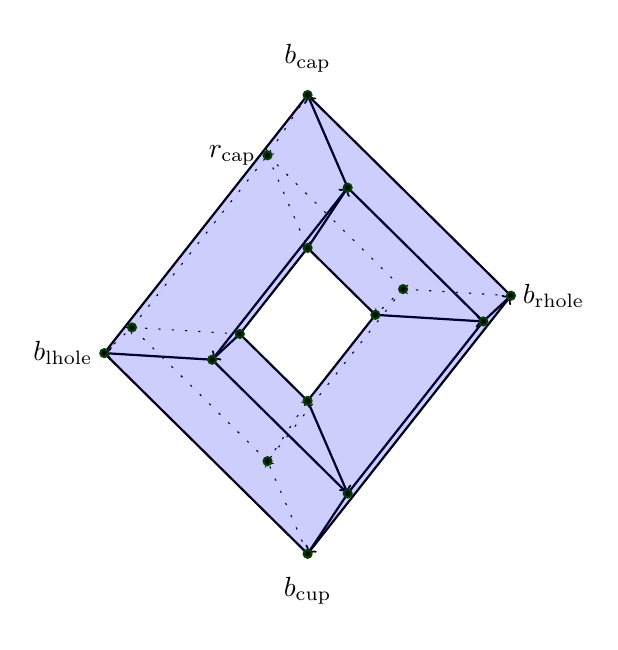
\begin{tikzpicture}%
  [x={(-0.860769cm, -0.121512cm)},
  y={(0.508996cm, -0.205391cm)},
  z={(-0.000053cm, 0.971107cm)},
  scale=1,
  back/.style={loosely dotted, thin},
  edge/.style={->,black, thick},
  line/.style={black, thick},
  facet/.style={fill=blue!95!black,fill opacity=0.1},
  vertex/.style={inner sep=1pt,circle,draw=green!25!black,fill=black,thick}]
\coordinate (r_cap) at (0, -1, 5);
\coordinate (g_cap) at (0, 0, 4 );
\coordinate (o_cap) at (0, 1, 5 );
\coordinate (b_cap) at (0, 0, 6 );

\coordinate (r_cup) at (0, -1, 1);
\coordinate (g_cup) at (0, 0, 2 );
\coordinate (o_cup) at (0, 1, 1 );
\coordinate (b_cup) at (0, 0, 0 );

\coordinate (r_ohole) at (-2, -1, 3);
\coordinate (g_ohole) at (-1, 0,  3);
\coordinate (o_ohole) at (-2, 1,  3);
\coordinate (b_ohole) at (-3, 0,  3);

\coordinate (r_rhole) at (2, -1, 3);
\coordinate (g_rhole) at (1, 0,  3);
\coordinate (o_rhole) at (2, 1,  3);
\coordinate (b_rhole) at (3, 0,  3);

\draw[edge,back] (r_cap) -- (g_cap);
\draw[edge]      (g_cap) -- (o_cap);
\draw[edge]      (o_cap) -- (b_cap);
\draw[edge,back] (b_cap) -- (r_cap);

\draw[edge,back] (r_cup) -- (g_cup);
\draw[edge]      (g_cup) -- (o_cup);
\draw[edge]      (o_cup) -- (b_cup);
\draw[edge,back] (b_cup) -- (r_cup);

\draw[edge,back] (r_ohole) -- (g_ohole);
\draw[edge]      (g_ohole) -- (o_ohole);
\draw[edge]      (o_ohole) -- (b_ohole);
\draw[edge,back] (b_ohole) -- (r_ohole);

\draw[edge,back] (r_rhole) -- (g_rhole);
\draw[edge]      (g_rhole) -- (o_rhole);
\draw[edge]      (o_rhole) -- (b_rhole);
\draw[edge,back] (b_rhole) -- (r_rhole);

\draw[line,back] (r_cap) --   (r_ohole);
\draw[line,back] (r_ohole) -- (r_cup);
\draw[line,back] (r_cup) --   (r_rhole);
\draw[line,back] (r_rhole) -- (r_cap);

\draw[line] (g_cap) --   (g_ohole);
\draw[line] (g_ohole) -- (g_cup);
\draw[line] (g_cup) --   (g_rhole);
\draw[line] (g_rhole) -- (g_cap);

\draw[line] (o_cap) --   (o_ohole);
\draw[line] (o_ohole) -- (o_cup);
\draw[line] (o_cup) --   (o_rhole);
\draw[line] (o_rhole) -- (o_cap);

\draw[line] (b_cap) --   (b_ohole);
\draw[line] (b_ohole) -- (b_cup);
\draw[line] (b_cup) --   (b_rhole);
\draw[line] (b_rhole) -- (b_cap);

\fill[facet] (r_cap) -- (r_ohole) -- (g_ohole) -- (g_cap) -- cycle {};
\fill[facet] (r_cap) -- (r_rhole) -- (g_rhole) -- (g_cap) -- cycle {};
\fill[facet] (r_cap) -- (r_ohole) -- (b_ohole) -- (b_cap) -- cycle {};
\fill[facet] (r_cap) -- (r_rhole) -- (b_rhole) -- (b_cap) -- cycle {};

\fill[facet] (o_cap) -- (o_ohole) -- (g_ohole) -- (g_cap) -- cycle {};
\fill[facet] (o_cap) -- (o_rhole) -- (g_rhole) -- (g_cap) -- cycle {};
\fill[facet] (o_cap) -- (o_ohole) -- (b_ohole) -- (b_cap) -- cycle {};
\fill[facet] (o_cap) -- (o_rhole) -- (b_rhole) -- (b_cap) -- cycle {};

\fill[facet] (r_cup) -- (r_ohole) -- (g_ohole) -- (g_cup) -- cycle {};
\fill[facet] (r_cup) -- (r_rhole) -- (g_rhole) -- (g_cup) -- cycle {};
\fill[facet] (r_cup) -- (r_ohole) -- (b_ohole) -- (b_cup) -- cycle {};
\fill[facet] (r_cup) -- (r_rhole) -- (b_rhole) -- (b_cup) -- cycle {};

\fill[facet] (o_cup) -- (o_ohole) -- (g_ohole) -- (g_cup) -- cycle {};
\fill[facet] (o_cup) -- (o_rhole) -- (g_rhole) -- (g_cup) -- cycle {};
\fill[facet] (o_cup) -- (o_ohole) -- (b_ohole) -- (b_cup) -- cycle {};
\fill[facet] (o_cup) -- (o_rhole) -- (b_rhole) -- (b_cup) -- cycle {};

\begin{scope}[nodes=vertex]
\node[label=left:\( r_{\mathrm{cap}} \)] at (r_cap) {};
\node at (g_cap) {};
\node at (o_cap) {};
\node[label=above:\( b_{\mathrm{cap}} \)] at (b_cap) {};
\node at (r_cup) {};
\node at (g_cup) {};
\node at (o_cup) {};
\node[label=below:\( b_{\mathrm{cup}} \)] at (b_cup) {};
\node at (r_ohole) {};
\node at (g_ohole) {};
\node at (o_ohole) {};
\node[label=right:\( b_{\mathrm{rhole}} \)] at (b_ohole) {};
\node at (r_rhole) {};
\node at (g_rhole) {};
\node at (o_rhole) {};
\node[label=left:\( b_{\mathrm{lhole}} \)] at (b_rhole) {};
\end{scope}
\end{tikzpicture}

\caption{Torus embedded in 3-dimensional space. If you see color in your rendering then black lines trace four square-shaped paths, red ones connect the front square to the middle diamonds, and blue ones connect the back path to the middle ones.}
\label{fig:torus}
\end{figure}

\begin{figure}[htbp]
\centering
% https://q.uiver.app/#q=WzAsMzYsWzEsNCwiXFxidWxsZXQiXSxbMSw2LCJcXGJ1bGxldCJdLFsyLDcsIlxcYnVsbGV0Il0sWzIsNSwiXFxidWxsZXQiXSxbMiwzLCJcXGJ1bGxldCJdLFsxLDgsIlxcYnVsbGV0Il0sWzEsMiwiXFxidWxsZXQiXSxbMywyLCJcXGJ1bGxldCJdLFszLDQsIlxcYnVsbGV0Il0sWzMsNiwiXFxidWxsZXQiXSxbMyw4LCJcXGJ1bGxldCJdLFsyLDEsIlxcYnVsbGV0Il0sWzQsMSwiXFxidWxsZXQiXSxbNSwyLCJcXGJ1bGxldCJdLFs0LDMsIlxcYnVsbGV0Il0sWzUsNCwiXFxidWxsZXQiXSxbNCw1LCJcXGJ1bGxldCJdLFs1LDYsIlxcYnVsbGV0Il0sWzQsNywiXFxidWxsZXQiXSxbNSw4LCJcXGJ1bGxldCJdLFsyLDAsIlxcbWF0aHJte2JhY2t9Il0sWzQsMCwiXFxtYXRocm17ZnJvbnR9Il0sWzEsMCwiXFxtYXRocm17b3V0ZXJ9Il0sWzMsMCwiXFxtYXRocm17aG9sZX0iXSxbNSwwLCJcXG1hdGhybXtvdXRlcn0iXSxbMSwxMCwiXFxidWxsZXQiXSxbMiw5LCJcXGJ1bGxldCJdLFszLDEwLCJcXGJ1bGxldCJdLFs0LDksIlxcYnVsbGV0Il0sWzUsMTAsIlxcYnVsbGV0Il0sWzAsMiwiXFxtYXRocm17dG9wXFwgb2ZcXCBkaWFtb25kc30iXSxbMCw2LCJcXG1hdGhybXtib3R0b21cXCBvZlxcIGRpYW1vbmRzfSJdLFsxLDEsIlxcICJdLFs1LDEsIlxcICJdLFszLDEsIlxcICJdLFswLDEwLCJcXG1hdGhybXt0b3BcXCBvZlxcIGRpYW1vbmRzfSJdLFs0LDMsIiIsMix7InN0eWxlIjp7ImhlYWQiOnsibmFtZSI6Im5vbmUifX19XSxbMywyLCIiLDIseyJzdHlsZSI6eyJoZWFkIjp7Im5hbWUiOiJub25lIn19fV0sWzAsMSwiIiwyLHsic3R5bGUiOnsiaGVhZCI6eyJuYW1lIjoibm9uZSJ9fX1dLFs0LDAsIiIsMSx7ImNvbG91ciI6WzIzNiw5MSw2MF0sInN0eWxlIjp7ImhlYWQiOnsibmFtZSI6Im5vbmUifX19XSxbMCwzLCIiLDEseyJjb2xvdXIiOlsyMzYsOTEsNjBdLCJzdHlsZSI6eyJoZWFkIjp7Im5hbWUiOiJub25lIn19fV0sWzMsMSwiIiwxLHsiY29sb3VyIjpbMjM2LDkxLDYwXSwic3R5bGUiOnsiaGVhZCI6eyJuYW1lIjoibm9uZSJ9fX1dLFsxLDIsIiIsMSx7ImNvbG91ciI6WzIzNiw5MSw2MF0sInN0eWxlIjp7ImhlYWQiOnsibmFtZSI6Im5vbmUifX19XSxbMiw1LCIiLDEseyJjb2xvdXIiOlsyMzYsOTEsNjBdLCJzdHlsZSI6eyJoZWFkIjp7Im5hbWUiOiJub25lIn19fV0sWzEsNSwiIiwxLHsic3R5bGUiOnsiaGVhZCI6eyJuYW1lIjoibm9uZSJ9fX1dLFs2LDQsIiIsMSx7ImNvbG91ciI6WzIzNiw5MSw2MF0sInN0eWxlIjp7ImhlYWQiOnsibmFtZSI6Im5vbmUifX19XSxbNiwwLCIiLDEseyJzdHlsZSI6eyJoZWFkIjp7Im5hbWUiOiJub25lIn19fV0sWzcsOCwiIiwwLHsic3R5bGUiOnsiaGVhZCI6eyJuYW1lIjoibm9uZSJ9fX1dLFs4LDksIiIsMCx7InN0eWxlIjp7ImhlYWQiOnsibmFtZSI6Im5vbmUifX19XSxbOSwxMCwiIiwwLHsic3R5bGUiOnsiaGVhZCI6eyJuYW1lIjoibm9uZSJ9fX1dLFs3LDQsIiIsMCx7ImNvbG91ciI6WzIzNiw5MSw2MF0sInN0eWxlIjp7ImhlYWQiOnsibmFtZSI6Im5vbmUifX19XSxbNCw4LCIiLDAseyJjb2xvdXIiOlsyMzYsOTEsNjBdLCJzdHlsZSI6eyJoZWFkIjp7Im5hbWUiOiJub25lIn19fV0sWzgsMywiIiwwLHsiY29sb3VyIjpbMjM2LDkxLDYwXSwic3R5bGUiOnsiaGVhZCI6eyJuYW1lIjoibm9uZSJ9fX1dLFszLDksIiIsMCx7ImNvbG91ciI6WzIzNiw5MSw2MF0sInN0eWxlIjp7ImhlYWQiOnsibmFtZSI6Im5vbmUifX19XSxbOSwyLCIiLDAseyJjb2xvdXIiOlsyMzYsOTEsNjBdLCJzdHlsZSI6eyJoZWFkIjp7Im5hbWUiOiJub25lIn19fV0sWzIsMTAsIiIsMCx7ImNvbG91ciI6WzIzNiw5MSw2MF0sInN0eWxlIjp7ImhlYWQiOnsibmFtZSI6Im5vbmUifX19XSxbMTEsNCwiIiwwLHsic3R5bGUiOnsiaGVhZCI6eyJuYW1lIjoibm9uZSJ9fX1dLFsxMSw2LCIiLDAseyJjb2xvdXIiOlsyMzYsOTEsNjBdLCJzdHlsZSI6eyJoZWFkIjp7Im5hbWUiOiJub25lIn19fV0sWzExLDcsIiIsMCx7ImNvbG91ciI6WzIzNiw5MSw2MF0sInN0eWxlIjp7ImhlYWQiOnsibmFtZSI6Im5vbmUifX19XSxbMTksMTcsIiIsMCx7InN0eWxlIjp7ImhlYWQiOnsibmFtZSI6Im5vbmUifX19XSxbMTgsMTYsIiIsMCx7InN0eWxlIjp7ImhlYWQiOnsibmFtZSI6Im5vbmUifX19XSxbMTYsMTQsIiIsMCx7InN0eWxlIjp7ImhlYWQiOnsibmFtZSI6Im5vbmUifX19XSxbMTcsMTUsIiIsMCx7InN0eWxlIjp7ImhlYWQiOnsibmFtZSI6Im5vbmUifX19XSxbMTUsMTMsIiIsMCx7InN0eWxlIjp7ImhlYWQiOnsibmFtZSI6Im5vbmUifX19XSxbMTQsMTIsIiIsMCx7InN0eWxlIjp7ImhlYWQiOnsibmFtZSI6Im5vbmUifX19XSxbMTIsNywiIiwwLHsiY29sb3VyIjpbMSw5NSw2MF0sInN0eWxlIjp7ImhlYWQiOnsibmFtZSI6Im5vbmUifX19XSxbMTIsMTMsIiIsMCx7ImNvbG91ciI6WzEsOTUsNjBdLCJzdHlsZSI6eyJoZWFkIjp7Im5hbWUiOiJub25lIn19fV0sWzEzLDE0LCIiLDAseyJjb2xvdXIiOlsxLDk1LDYwXSwic3R5bGUiOnsiaGVhZCI6eyJuYW1lIjoibm9uZSJ9fX1dLFsxNCw4LCIiLDAseyJjb2xvdXIiOlsxLDk1LDYwXSwic3R5bGUiOnsiaGVhZCI6eyJuYW1lIjoibm9uZSJ9fX1dLFsxNCwxNSwiIiwwLHsiY29sb3VyIjpbMSw5NSw2MF0sInN0eWxlIjp7ImhlYWQiOnsibmFtZSI6Im5vbmUifX19XSxbMTUsMTYsIiIsMCx7ImNvbG91ciI6WzEsOTUsNjBdLCJzdHlsZSI6eyJoZWFkIjp7Im5hbWUiOiJub25lIn19fV0sWzgsMTYsIiIsMCx7ImNvbG91ciI6WzEsOTUsNjBdLCJzdHlsZSI6eyJoZWFkIjp7Im5hbWUiOiJub25lIn19fV0sWzE2LDksIiIsMCx7ImNvbG91ciI6WzEsOTUsNjBdLCJzdHlsZSI6eyJoZWFkIjp7Im5hbWUiOiJub25lIn19fV0sWzE2LDE3LCIiLDAseyJjb2xvdXIiOlsxLDk1LDYwXSwic3R5bGUiOnsiaGVhZCI6eyJuYW1lIjoibm9uZSJ9fX1dLFsxNywxOCwiIiwwLHsiY29sb3VyIjpbMSw5NSw2MF0sInN0eWxlIjp7ImhlYWQiOnsibmFtZSI6Im5vbmUifX19XSxbOSwxOCwiIiwwLHsiY29sb3VyIjpbMSw5NSw2MF0sInN0eWxlIjp7ImhlYWQiOnsibmFtZSI6Im5vbmUifX19XSxbMTgsMTksIiIsMCx7ImNvbG91ciI6WzEsOTUsNjBdLCJzdHlsZSI6eyJoZWFkIjp7Im5hbWUiOiJub25lIn19fV0sWzE4LDEwLCIiLDAseyJjb2xvdXIiOlsxLDk1LDYwXSwic3R5bGUiOnsiaGVhZCI6eyJuYW1lIjoibm9uZSJ9fX1dLFs3LDE0LCIiLDAseyJjb2xvdXIiOlsxLDk1LDYwXSwic3R5bGUiOnsiaGVhZCI6eyJuYW1lIjoibm9uZSJ9fX1dLFs1LDI2LCIiLDEseyJjb2xvdXIiOlsyMzYsOTEsNjBdLCJzdHlsZSI6eyJoZWFkIjp7Im5hbWUiOiJub25lIn19fV0sWzEwLDI2LCIiLDEseyJjb2xvdXIiOlsyMzYsOTEsNjBdLCJzdHlsZSI6eyJoZWFkIjp7Im5hbWUiOiJub25lIn19fV0sWzIsMjYsIiIsMSx7InN0eWxlIjp7ImhlYWQiOnsibmFtZSI6Im5vbmUifX19XSxbMTgsMjgsIiIsMSx7InN0eWxlIjp7ImhlYWQiOnsibmFtZSI6Im5vbmUifX19XSxbMjYsMjUsIiIsMSx7ImNvbG91ciI6WzIzNiw5MSw2MF0sInN0eWxlIjp7ImhlYWQiOnsibmFtZSI6Im5vbmUifX19XSxbMjYsMjcsIiIsMSx7ImNvbG91ciI6WzIzNiw5MSw2MF0sInN0eWxlIjp7ImhlYWQiOnsibmFtZSI6Im5vbmUifX19XSxbMjgsMjksIiIsMSx7ImNvbG91ciI6WzEsOTUsNjBdLCJzdHlsZSI6eyJoZWFkIjp7Im5hbWUiOiJub25lIn19fV0sWzE5LDI5LCIiLDEseyJzdHlsZSI6eyJoZWFkIjp7Im5hbWUiOiJub25lIn19fV0sWzEwLDI3LCIiLDEseyJzdHlsZSI6eyJoZWFkIjp7Im5hbWUiOiJub25lIn19fV0sWzUsMjUsIiIsMSx7InN0eWxlIjp7ImhlYWQiOnsibmFtZSI6Im5vbmUifX19XSxbMjgsMjcsIiIsMSx7ImNvbG91ciI6WzEsOTUsNjBdLCJzdHlsZSI6eyJoZWFkIjp7Im5hbWUiOiJub25lIn19fV0sWzI4LDE5LCIiLDEseyJjb2xvdXIiOlsxLDk1LDYwXSwic3R5bGUiOnsiaGVhZCI6eyJuYW1lIjoibm9uZSJ9fX1dLFsyOCwxMCwiIiwxLHsiY29sb3VyIjpbMSw5NSw2MF0sInN0eWxlIjp7ImhlYWQiOnsibmFtZSI6Im5vbmUifX19XSxbMzAsNiwiIiwxLHsic3R5bGUiOnsiYm9keSI6eyJuYW1lIjoiZG90dGVkIn19fV0sWzMxLDEsIiIsMSx7InN0eWxlIjp7ImJvZHkiOnsibmFtZSI6ImRvdHRlZCJ9fX1dLFsyMCwxMSwiIiwwLHsic3R5bGUiOnsiYm9keSI6eyJuYW1lIjoiZG90dGVkIn19fV0sWzIxLDEyLCIiLDAseyJzdHlsZSI6eyJib2R5Ijp7Im5hbWUiOiJkb3R0ZWQifX19XSxbMjIsMzIsIiIsMCx7InN0eWxlIjp7ImJvZHkiOnsibmFtZSI6ImRvdHRlZCJ9fX1dLFsyNCwzMywiIiwwLHsic3R5bGUiOnsiYm9keSI6eyJuYW1lIjoiZG90dGVkIn19fV0sWzIzLDM0LCIiLDAseyJzdHlsZSI6eyJib2R5Ijp7Im5hbWUiOiJkb3R0ZWQifX19XSxbMzUsMjUsIiIsMSx7InN0eWxlIjp7ImJvZHkiOnsibmFtZSI6ImRvdHRlZCJ9fX1dXQ==
\begin{tikzcd}[column sep=1ex,row sep=1ex]
	& {\mathrm{outer}} & {\mathrm{back}} & {\mathrm{hole}} & {\mathrm{front}} & {\mathrm{outer}} \\
	& {\ } & \bullet & {\ } & \bullet & {\ } \\
	{\mathrm{top\ of\ diamonds}} & \bullet && \bullet && \bullet \\
	&& \bullet && \bullet \\
	& \bullet && \bullet && \bullet \\
	&& \bullet && \bullet \\
	{\mathrm{bottom\ of\ diamonds}} & \bullet && \bullet && \bullet \\
	&& \bullet && \bullet \\
	& \bullet && \bullet && \bullet \\
	&& \bullet && \bullet \\
	{\mathrm{top\ of\ diamonds}} & \bullet && \bullet && \bullet
	\arrow[dotted, from=1-2, to=2-2]
	\arrow[dotted, from=1-3, to=2-3]
	\arrow[dotted, from=1-4, to=2-4]
	\arrow[dotted, from=1-5, to=2-5]
	\arrow[dotted, from=1-6, to=2-6]
	\arrow[draw={rgb,255:red,60;green,73;blue,246}, no head, from=2-3, to=3-2]
	\arrow[draw={rgb,255:red,60;green,73;blue,246}, no head, from=2-3, to=3-4]
	\arrow[no head, from=2-3, to=4-3]
	\arrow[draw={rgb,255:red,250;green,59;blue,56}, no head, from=2-5, to=3-4]
	\arrow[draw={rgb,255:red,250;green,59;blue,56}, no head, from=2-5, to=3-6]
	\arrow[dotted, from=3-1, to=3-2]
	\arrow[draw={rgb,255:red,60;green,73;blue,246}, no head, from=3-2, to=4-3]
	\arrow[no head, from=3-2, to=5-2]
	\arrow[draw={rgb,255:red,60;green,73;blue,246}, no head, from=3-4, to=4-3]
	\arrow[draw={rgb,255:red,250;green,59;blue,56}, no head, from=3-4, to=4-5]
	\arrow[no head, from=3-4, to=5-4]
	\arrow[draw={rgb,255:red,250;green,59;blue,56}, no head, from=3-6, to=4-5]
	\arrow[draw={rgb,255:red,60;green,73;blue,246}, no head, from=4-3, to=5-2]
	\arrow[draw={rgb,255:red,60;green,73;blue,246}, no head, from=4-3, to=5-4]
	\arrow[no head, from=4-3, to=6-3]
	\arrow[no head, from=4-5, to=2-5]
	\arrow[draw={rgb,255:red,250;green,59;blue,56}, no head, from=4-5, to=5-4]
	\arrow[draw={rgb,255:red,250;green,59;blue,56}, no head, from=4-5, to=5-6]
	\arrow[draw={rgb,255:red,60;green,73;blue,246}, no head, from=5-2, to=6-3]
	\arrow[no head, from=5-2, to=7-2]
	\arrow[draw={rgb,255:red,60;green,73;blue,246}, no head, from=5-4, to=6-3]
	\arrow[draw={rgb,255:red,250;green,59;blue,56}, no head, from=5-4, to=6-5]
	\arrow[no head, from=5-4, to=7-4]
	\arrow[no head, from=5-6, to=3-6]
	\arrow[draw={rgb,255:red,250;green,59;blue,56}, no head, from=5-6, to=6-5]
	\arrow[draw={rgb,255:red,60;green,73;blue,246}, no head, from=6-3, to=7-2]
	\arrow[draw={rgb,255:red,60;green,73;blue,246}, no head, from=6-3, to=7-4]
	\arrow[no head, from=6-3, to=8-3]
	\arrow[no head, from=6-5, to=4-5]
	\arrow[draw={rgb,255:red,250;green,59;blue,56}, no head, from=6-5, to=7-4]
	\arrow[draw={rgb,255:red,250;green,59;blue,56}, no head, from=6-5, to=7-6]
	\arrow[dotted, from=7-1, to=7-2]
	\arrow[draw={rgb,255:red,60;green,73;blue,246}, no head, from=7-2, to=8-3]
	\arrow[no head, from=7-2, to=9-2]
	\arrow[draw={rgb,255:red,60;green,73;blue,246}, no head, from=7-4, to=8-3]
	\arrow[draw={rgb,255:red,250;green,59;blue,56}, no head, from=7-4, to=8-5]
	\arrow[no head, from=7-4, to=9-4]
	\arrow[no head, from=7-6, to=5-6]
	\arrow[draw={rgb,255:red,250;green,59;blue,56}, no head, from=7-6, to=8-5]
	\arrow[draw={rgb,255:red,60;green,73;blue,246}, no head, from=8-3, to=9-2]
	\arrow[draw={rgb,255:red,60;green,73;blue,246}, no head, from=8-3, to=9-4]
	\arrow[no head, from=8-3, to=10-3]
	\arrow[no head, from=8-5, to=6-5]
	\arrow[draw={rgb,255:red,250;green,59;blue,56}, no head, from=8-5, to=9-4]
	\arrow[draw={rgb,255:red,250;green,59;blue,56}, no head, from=8-5, to=9-6]
	\arrow[no head, from=8-5, to=10-5]
	\arrow[color={rgb,255:red,60;green,73;blue,246}, no head, from=9-2, to=10-3]
	\arrow[no head, from=9-2, to=11-2]
	\arrow[color={rgb,255:red,60;green,73;blue,246}, no head, from=9-4, to=10-3]
	\arrow[no head, from=9-4, to=11-4]
	\arrow[no head, from=9-6, to=7-6]
	\arrow[no head, from=9-6, to=11-6]
	\arrow[color={rgb,255:red,60;green,73;blue,246}, no head, from=10-3, to=11-2]
	\arrow[color={rgb,255:red,60;green,73;blue,246}, no head, from=10-3, to=11-4]
	\arrow[color={rgb,255:red,250;green,59;blue,56}, no head, from=10-5, to=9-4]
	\arrow[color={rgb,255:red,250;green,59;blue,56}, no head, from=10-5, to=9-6]
	\arrow[color={rgb,255:red,250;green,59;blue,56}, no head, from=10-5, to=11-4]
	\arrow[color={rgb,255:red,250;green,59;blue,56}, no head, from=10-5, to=11-6]
	\arrow[dotted, from=11-1, to=11-2]
\end{tikzcd}

\caption{An inspiration for the torus. Identify the sides and then the top, definitionally, to get the actual torus.}
\label{fig:flattorus}
\end{figure}

This somewhat arbitrary and unfamiliar model of a torus has the helpful property that it is a combinatorial manifold that is somewhat minimal while still being representable by a donut shape. But the donut-shaped version suggests a very different connection than the flat model! Starting with the flat model, we can easily see how to define \( T_1 \) by sliding a link rigidly along the page to the link of some adjacent vertex. Then we can see that transport around any loop is the identity and so \( T_2 \) is always the identity (together with the homotopy \( \refl_\id \) from the identity to itself). So if we imagine a way to visit every face like we did for the octahedron, starting and ending at some basepoint \( v \), we expect to see no net rotation at all of \( Tv \). Later we will call this ``total curvature 0.''

The donut-shaped torus suggests a different connection, one determined by the embedding in 3-space that we have represented. But the easiest way to think about that bundle and its connection and curvature is to wait until we have a proof of the Poincaré-Hopf theorem, so that we can instead compute with a vector field.
\end{comment}

\subsection{Existence of connections}

How confident can we be that we can always define a connection on an arbitrary combinatorial manifold? Two things make the octahedron example special: the link is a 4-gon at every vertex, and every edge extends to a symmetry of the entire octahedron, embedded in 3-dimensional space. This imposed a coherence on the interactions of all the choices we made for the connection, which we can worry may not exist for more complex combinatorial data.

We know as a fact outside of HoTT that any combinatorial surface that has been realized as a triangulated surface embedded in 3-dimensional euclidean space can inherit the parallel transport entailed in the embedding. We could then approximate that data to arbitrary precision with enough subdivision of the fibers of \( T \).

What would a proof inside of HoTT look like? We will leave this as an open question.



\section{Why this works}

\subsection{Classical connections}

\begin{mydef}
A \defemph{principal bundle} is a smooth map \( \pi:P\to M \) between smooth manifolds such that
\begin{enumerate}
\item All the fibers of \( \pi \) are equivalent as a smooth manifold to a fixed Lie group \( G \).
\item There is a smooth \( G \)-action \( P\times G\to P \) on the right that acts on fibers, and does so freely and transitively.
\item There exists an open cover \( \{U_i\} \) of \( M \) and equivariant diffeomorphisms \( \phi_i:P|_{U_i}\to U_i\times G \) (i.e. \( \phi_i(p\cdot g)= \phi_i(p)\cdot g\)).
\end{enumerate}
\end{mydef}

Physicists call principal bundle automorphisms ``gauge transformations'':

\begin{mydef}
A \defemph{gauge transformation} is a map \( \Phi:P\to P \) commuting with the projection to \( M \) and which is \( G \)-equivariant, i.e. \( \Phi(p\cdot g) = \Phi(p)\cdot g \). Denote the group of gauge transformations by \( \Aut P \). In the literature it is sometimes denoted \( \mathscr{G}(P) \).
\end{mydef}

\begin{mydef}
The \defemph{vertical bundle} \( VP \) of a principal bundle \( \pi:P\to M \) with Lie group \( G \) is the kernel of the derivative \( T\pi:TP\to TM \).
\end{mydef}

\( VP \) can be visualized as the collection of tangent vectors that point along the fibers. It should be clear that at each point of \( M \) the group \( G \) acts on \( VP \), sending vertical vectors to vertical vectors. In other words, \( \Aut P \) acts on \( VP \).

\begin{mydef}
An \defemph{Ehresmann connection} on a principal bundle \( \pi:P\to M \) with Lie group \( G \) is a splitting \( TP=VP\oplus HP \) at every point of \( P \) into vertical and complementary ``horizontal'' subspaces, which is preserved by the action of \( \Aut P \).
\end{mydef}

Being preserved by the action of \( \Aut P \) implies that the complementary horizontal subspaces in a given fiber of \( \pi:P\to M \) are determined by the splitting at any single point in the fiber. The action of \( G \) on this fiber can then push the splitting around to all the other points.

The utility and parsimony of this definition relates to the solvability of ordinary differential equations. We now have an isomorphism \( T_p\pi:H_pP\simeq T_{\pi(p)}M \) between each horizontal space and the tangent space below it in \( M \). This means that given a tangent vector at \( x:M \) and a point \( p \) in \( \pi^{-1}(x) \) we can uniquely lift the tangent vector to a horizontal vector at \( p \). We can also lift vector fields and paths in this way. To lift a path \( \gamma:[0,1]\to M \) you must specify a lift for \( \gamma(0) \) and then lift the tangent vectors of \( \gamma \) and prove that you can integrate the lift of that vector field upstairs in \( HP \).

Armed with the lifting of paths one immediately obtains isomorphisms between the fibers of \( P \): given a path in \( M \) we can map the starting point of a lift to the ending point. So the three constructions: the Ehresmann connection, the lifting of paths, and transport isomorphisms between fibers are all recapitulations of the structure that the connection adds to the bundle.

\subsubsection{Gauge theory}

Given a bundle \( \pi:P\to M \) there is a space of connections \( \mathscr{A}(P) \). The group \( \Aut P \) acts on this space. For example, a gauge transformation that is constant in the neighborhood of a point will not change the splitting, it will just shift the fiber rigidly along itself. But at the other extreme, a gauge transformation that is changing rapidly near a point will tilt the horizontal subspaces rapidly. The field of \defemph{gauge theory} begins with a study of the quotient space \( \mathscr{A}(P)/\Aut P \).

\begin{mynote}
Recall that torsors have a physical interpretation as a quantity without a specified unit, such as mass, length, or time. When we choose a base point in a torsor it becomes the standard torsor \( G \) acting on itself (for example, the additive real numbers). A physicist is looking for properties or laws that are independent of such a choice. In the 20th century physicists further wondered about choices of units that vary from point to point, and began searching for laws that are invariant under this much larger space of transformations. This led directly to the discovery of connections and curvature as useful fields that complement the matter fields, which are sections of associated vector bundles. They were then led to explore quotienting by the action of the group of gauge transformations, and in particular the space of connections ``mod gauge.'' In this scenario the base manifold \( M \) is spacetime, and a gauge transformation is a smoothly varying choice of gauge (units) at each point.
\end{mynote}

We can characterize connections and curvature in terms of splittings of certain sequences. Atiyah and Bott (\cite{atiyah1983yang} equation 3.4) describe the space of vector fields on a total space \( P \) as a Lie algebra extension of \( \Gamma TM \) by \( \Gamma \ad P \), respectively the Lie algebra of vector fields on the base and vertical vector fields on \( P \). A non-flat connection will fail to split this sequence because horizontal vector fields may have a non-horizontal component when taking the Lie bracket. This extension is referred to as the \emph{Atiyah sequence}. 

In this century mathematicians in HoTT and HoTT-adjacent fields sought an \emph{integrated Atiyah sequence}, including Urs Schreiber\cite{urs_atiyah}\cite{urs_atiyah_blog}. This would be a Lie groupoidal version of the Atiyah sequence on Lie algebras. If a groupoid extension could be examined, a link could be sought to Schreier theory. We'll return to these ideas in the next section.

\subsection{Type theory version}

Moving now to HoTT, fix a type \( M:\U \) and a type family \( f:M\to\U \). Path induction gives us the transport isomorphism \( \pit{p:a=_M b}\tr(p):f(a)=f(b) \). We can use this to define a type of \emph{dependent paths}, also called \emph{pathovers} or \emph{paths over} a given path.

\begin{mydef}
With the above context and points \( \alpha:f(a), \beta:f(b) \) the type of \defemph{dependent paths over \( p \)} with endpoints \( \alpha, \beta \) is denoted
\[ \alpha\pathover{p}\beta.
\]
By induction we can assume \( p \) is \( \refl_a \) in which case \( \alpha\pathover{p}\beta \) is \( \alpha=_{f(a)}\alpha \).
\end{mydef}

See \cite{Symmetry} for more discussion of dependent paths (where they use the term ``path over''), including composition, and associativity thereof.

We recall now the identity type of sigma types:

\begin{mythm}\label{thm:idsit}
(HoTT book Theorem 2.7.2 \cite{hottbook}) If \( f:M\to \U \) is a type family and \( \alpha,\beta:\sit{x:M}f(x) \) then there is an equivalence 
\[ 
\mathsf{split}:(\alpha=\beta)\simeq \sit{p:\pr_1(\alpha)=_M\pr_1(\beta)} \left[\tr(p)(\pr_2(\alpha))\right] = \pr_2(\beta).
\]
\end{mythm}

\begin{mydef}
Given \( p:a=_M b \) and \( \alpha:f(a) \) we have 
\[
\left(\alpha\pathover{p}\tr(p)(\alpha)\right)\simeq \left(\tr(p)(\alpha)=_{f(b)}\tr(p)(\alpha)\right)
\]
which has the term \( \refl \) which we can call \defemph{the horizontal lift of \( p \) starting at \( \alpha \)}.
\end{mydef}

 We can imitate the classical definition of a connection by defining \( \omega\defeq \pr_2\circ\mathsf{split} \), the projection onto the vertical component.

In HoTT if the bundle is classified by \( f:M\to \U \) then an automorphism is a homotopy \( H:f\sim f \) and the group of gauge transformations is the loop space \( \Omega_f(M\to \U) \). What is the effect of applying a homotopy \( H:f\sim f \) on transport, and on splitting?

\( H \) is a family of fiber automorphisms: \( H:\pit{a:M}f(a)=f(a) \) which we can assemble into an equivalence \( H':\sit{a:M}f(a)=\sit{a:M}f(a) \) that acts fiberwise. We want to compute the action of \( \ap(H') \) on the horizontal-vertical decomposition of paths from Theorem~\ref{thm:idsit} by computing \( \omega\circ\ap(H')=\pr_2\circ\mathsf{split}\circ\ap(H') \).

Denote \( \sit{a:M}f(a) \) by \( P \). Let \( p:a=_M b \) be a path in the base and let \( \pi:(a,\alpha)=_P (b,\beta) \) be a path in \( P \) over \( p \). Then \( \omega(\pi):\tr_p(\alpha)=\beta \).

Now let's apply \( H \). We have \( \ap(H')(\pi):(a,H(a)(\alpha))=_P(b,H(b)(\beta)) \) which is still a path over \( p \). Applying \( \omega \) we get \[ \omega(\ap(H')(\pi)):\tr_p(H(a)(\alpha))=(H(b)(\beta)). \] Using the lemma below we can if we wish rewrite this as 
\[ 
\omega(\ap(H')(\pi)):H(b)\left[\tr_p(\alpha)=\beta\right]
\]
which uses only \( H(b) \). This is the action of gauge transformations on connections.

\begin{mylemma}
Given a function \( f:M\to\U \), path \( p:a=_M b \), and homotopy \( H:f\sim f \) the following square commutes and so in the type family we have \( \tr(H(x)\cdot f(p)) = \tr(f(p)\cdot H(y)) \).
\end{mylemma}
\begin{center}
% https://q.uiver.app/#q=WzAsNCxbMCwwLCJmKGEpIl0sWzEsMCwiZihiKSJdLFsxLDEsImYoYikiXSxbMCwxLCJmKGEpIl0sWzAsMywiSChhKSIsMix7InN0eWxlIjp7ImhlYWQiOnsibmFtZSI6Im5vbmUifX19XSxbMCwxLCJmKHApIiwwLHsic3R5bGUiOnsiaGVhZCI6eyJuYW1lIjoibm9uZSJ9fX1dLFszLDIsImYocCkiLDIseyJzdHlsZSI6eyJoZWFkIjp7Im5hbWUiOiJub25lIn19fV0sWzEsMiwiSChiKSIsMCx7InN0eWxlIjp7ImhlYWQiOnsibmFtZSI6Im5vbmUifX19XV0=
\begin{tikzcd}
  {f(a)} & {f(b)} \\
  {f(a)} & {f(b)}
  \arrow["{f(p)}", equal, from=1-1, to=1-2]
  \arrow["{H(a)}"', equal, from=1-1, to=2-1]
  \arrow["{H(b)}", equal, from=1-2, to=2-2]
  \arrow["{f(p)}"', equal, from=2-1, to=2-2]
\end{tikzcd}
\end{center}

HoTT provides new ways to talk about trivializations of bundles, and flatness of connections.

\begin{mythm}\label{thm:triv}
The following are equivalent for a map \( T:M\to\EMzo \):
\begin{enumerate}
\item The principal bundle \( P\defeq\sit{x:M}Tx \) is a trivial bundle.
\item The dependent sum \( \sit{x:M}Tx \) is equivalent to a non-dependent sum.
\item There exists a total lifting \( T_\bullet \) to pointed types.
\item \( T \) is contractible.
\end{enumerate}
\end{mythm}

\begin{proof}
1 and 2 are equivalent by definition. 1 implies 3 by choosing the basepoint of the second factor of \( M\times \so \). 3 implies 1 because the global choice of basepoint is a global isomorphism with \( \so \). 1 and 4 are equivalent because a trivialization is a contraction to \( M\times\so \).
\end{proof}

The classical definition of a flat connection is that contractible loops lift to horizontal loops, i.e. there is no holonomy around small loops. This implies that homotopic paths have the same transport. Here's how we'll describe this in HoTT:
\begin{mydef}
We call a connection on \( \sit{x:M}Tx \) \defemph{flat} if \( T \) factors through the 1-truncation \( ||M||_1 \).
\end{mydef}

\begin{mylemma}
If \( T:M\to\EMzo \) is flat and \( M \) is simply connected then \( T \) is trivial.
\end{mylemma}
\begin{proof}
\( T \) factors through \( ||M||_1 \) which is contractible.
\end{proof}

\subsubsection{Gauge theory revisited}

The sigma type \( P\defeq\sit{x:M}Tx \) and projection map to \( M \) package the insights of the Atiyah sequence and observations about what does and doesn't split:

The fiber sequence \( \so\to P\to M \) does not split unless \( P \) is trivial, by Theorem~\ref{thm:triv}.

Paths \( p:a=_M b \) do lift to \( P \) given a starting point \( \alpha:Ta \). This is what we are calling the connection, and it is the finite version of the vertical/horizontal splitting \( TP=VP\oplus HP \). Theorem~\ref{thm:idsit} provides the factoring of pathovers into horizontal and vertical. So at the level of paths there \emph{is} a splitting, a map from \( M \) to \( P \).

But suppose we have two paths \( p,q:a=_M b \) and a point \( \alpha \) over \( a \). If we concatenate the two horizontal lifts \( (p,\refl_{\tr(p)(\alpha)}) \) and \( (q^{-1}, \refl_{\tr(q^{-1})\circ\tr(p)(\alpha)}) \) into a loopover of \( p\cdot q^{-1} \) then we get a term in \( (p\cdot q^{-1}, \tr(q^{-1})\circ\tr(p)(\alpha)=\alpha) \). As we have seen this can be a non-\( \refl \) path in \( Ta \)! The concatenation of two horizontal lifts can be non-horizontal. This is the analogous statement to Atiyah's observation that the Lie bracket of two horizontal vectors can have a vertical component, and that this can be identified with curvature.

To work with connections mod gauge we don't really have to add anything to our existing picture, because we are always working with higher types such as \( M\to\EMzo \) which have automorphisms (in this case gauge transformations, aka self-homotopies) baked in.

Thinking back to the desired link with Schreier theory, David Jaz Myers showed that in the case of higher groups we have an equivalence between the type of extensions of a group \( G \) by \( F \) and the actions of \( G \) on a delooping \( BF \):
\[ 
\mathrm{Ext}(G; F) \simeq (BG \dotto \BAut(BF))
\]
(see \cite{myersthesis} Theorem 2.5.7). Our type of classifying maps \( M\to\EMzo \) can be seen as extensions of \( \pi_1(M) \), or of \( M \) itself, by the group \( \so \). What a lovely reframing of principal bundles.

\subsection{The Leibniz (product) rule}

The intuition that motivates everything in this note is that derivatives and connections are visible in type theory through the action on paths, because a path is a finite version of an infinitesimal tangent vector. And if we think we have some new understanding of differentiation, then we should be able to see the Leibniz rule.

The Leibniz rule, or product rule, for differentiation states that if \( f, g:M\to \rr \) are two smooth functions to the real numbers then \( d(fg) = fdg + gdf \). Here \( fg \) is the function formed by taking the pointwise product of \( f \) and \( g \). This is an interaction between multiplication in \( \rr \) and the action on vectors of smooth functions (the 1-forms \( df \) and \( dg \)). 

To examine this situation in HoTT we need type-theoretic functions \( f, g:M\to B \) from some type \( M \) to a central H-space \( B \). Let \( \mu:B\to B\to B \) be the H-space multiplication. How does \( \mu \) act on paths? Suppose we have \( a, a', b, b':B \) and \( p:a=_B a', q:b=_B b' \). Then we also have homotopies \( \mu(p, -):\mu(a, -)=_{B\to B}\mu(a', -) \) and \( \mu(-,q):\mu(-,b)=_{B\to B}\mu(-,b'). \) Since \( \mu(a, -):B=B \) is an (unpointed) equivalence of \( B \), and similarly for \( \mu(b, -) \) and so on, this data assembles into the following diagram of higher groupoid morphisms:

\begin{center}
% https://q.uiver.app/#q=WzAsMyxbMiwwLCJCIl0sWzAsMCwiQiJdLFs0LDAsIkIiXSxbMSwwLCJcXG11KGEsLSkiLDAseyJjdXJ2ZSI6LTN9XSxbMSwwLCJcXG11KGEnLC0pIiwyLHsiY3VydmUiOjN9XSxbMCwyLCJcXG11KC0sYikiLDAseyJjdXJ2ZSI6LTN9XSxbMCwyLCJcXG11KC0sYicpIiwyLHsiY3VydmUiOjN9XSxbMyw0LCJcXG11KHAsLSkiLDIseyJzaG9ydGVuIjp7InNvdXJjZSI6MjAsInRhcmdldCI6MjB9fV0sWzUsNiwiXFxtdSgtLHEpIiwyLHsic2hvcnRlbiI6eyJzb3VyY2UiOjIwLCJ0YXJnZXQiOjIwfX1dXQ==
\begin{tikzcd}
  B && B && B
  \arrow[""{name=0, anchor=center, inner sep=0}, "{\mu(a,-)}", curve={height=-18pt}, from=1-1, to=1-3]
  \arrow[""{name=1, anchor=center, inner sep=0}, "{\mu(a',-)}"', curve={height=18pt}, from=1-1, to=1-3]
  \arrow[""{name=2, anchor=center, inner sep=0}, "{\mu(-,b)}", curve={height=-18pt}, from=1-3, to=1-5]
  \arrow[""{name=3, anchor=center, inner sep=0}, "{\mu(-,b')}"', curve={height=18pt}, from=1-3, to=1-5]
  \arrow["{\mu(p,-)}"', shorten <=5pt, shorten >=5pt, Rightarrow, from=0, to=1]
  \arrow["{\mu(-,q)}"', shorten <=5pt, shorten >=5pt, Rightarrow, from=2, to=3]
\end{tikzcd}
\end{center}

And so the two homotopies can be horizontally composed to give a path \[ \mu(p,-)\star\mu(-,q): \mu(a, b)=\mu(a',b'). \] Horizontal composition is given by \[\mu(p,-)\star\mu(-,q)\defeq(\mu(p,-)\cdot_r \mu(-,b))\cdot(\mu(a', -)\cdot_l\mu(-, q))\] where \[ \mu(p,-)\cdot_r\mu(-,b):\mu(a,b)=\mu(a',b) \] and \[ \mu(a',-)\cdot_l\mu(-,q):\mu(a',b)=\mu(a',b') \] are defined by path induction.  See the HoTT book Theorem 2.1.6 on the Eckmann-Hilton argument\cite{hottbook}.

We can recognize the process of using whiskering to form horizontal composition in the Leibniz rule. 

Quick aside: moving from infinitesimal calculus to finite groupoid algebra actually involves two changes. The first is the change from vectors to paths, forms to functions and so on. But it's also the case that tangent vectors have just the one basepoint, whereas paths have two endpoints. You can see this play out in this example, where \( a \) and \( a' \) were distinct points (and \( b \) and \( b' \)).

The horizontal composition we build lives entirely in \( B \) and we didn't make use of \( M \) yet. The Leibniz rule will be a pointwise version of what's going on in \( B \). Denote by \( \mu\circ(f,g):M\to B \) the map which sends \( x\mapsto \mu(f(x),g(x)) \).

\begin{mylemma}
Given \( f, g:M\to B \) and \( p:x=_M y \) then 
\begin{align*}
 \ap(\mu\circ(f,g))(p)&=\mu(f(p),-)\star\mu(-,g(p))\\
 &=\left[\mu(f(p),-)\cdot_r \mu(-,g(x))\right]\cdot \left[\mu(f(y),-)\cdot_l\mu(-,g(p))\right]\\
 &:\mu(f(x),g(x))=\mu(f(y),g(y))
\end{align*}
\end{mylemma}



\bibliography{connections}
\end{document}



